% ============================================================
%  The Particle Model — Experiment Booklet (one section per experiment)
%  Year 7 (Year 8 extension)  |  Victorian Curriculum F–10 Version 2.0
%  Compile with: xelatex three times, then python3 fill.py Particle_Model_Experiment_Booklet_Yr7
% ============================================================
\documentclass[11pt,a4paper]{article}
\newcommand{\unitname}{The Particle Model}\newcommand{\unitcaps}{THE PARTICLE MODEL}

% ── Fonts (compile with LuaLaTeX) ────────────────────────────────────────────
\usepackage{fontspec}
% Bundled fonts (in ./fonts/) so the document compiles anywhere with XeLaTeX/LuaLaTeX
\setmainfont{Lato}[                   % body — humanist sans (stands in for deck's Inter)
  Path=./fonts/, Extension=.ttf, Ligatures=TeX,
  UprightFont=Lato-Regular, ItalicFont=Lato-Italic,
  BoldFont=Lato-Bold, BoldItalicFont=Lato-BoldItalic ]
\newfontfamily\headingfont{Poppins}[  % display/headings — matches the slide decks
  Path=./fonts/, Extension=.ttf, Ligatures=TeX,
  UprightFont=Poppins-Regular, ItalicFont=Poppins-Italic,
  BoldFont=Poppins-Bold, BoldItalicFont=Poppins-BoldItalic ]
\setlength{\headheight}{22pt}

\usepackage[protrusion=true,expansion=false]{microtype}
\usepackage[a4paper, top=2cm, bottom=2cm, left=2cm, right=2cm]{geometry}
\usepackage{xcolor}
\usepackage{tikz}
\usetikzlibrary{arrows.meta, shapes.geometric, calc, positioning, decorations.pathreplacing}
\usepackage{tcolorbox}
\tcbuselibrary{skins, breakable, raster}
\usepackage{fancyhdr}
\usepackage{titlesec}
\usepackage{enumitem}
\usepackage{booktabs}
\usepackage{tabularx}
\usepackage{array}
\usepackage{colortbl}
\usepackage{multicol}
\usepackage{amsmath}
\usepackage{needspace}
% TikZ diagram macros are embedded below (just before \begin{document}) for easy editing.
\usepackage{longtable}
\usepackage{lastpage}
\usepackage{calc}
\usepackage{mdframed}
\usepackage{setspace}
\usepackage{ragged2e}
% PDF bookmarks: one per lesson (made in \sectiondiv) plus the cover and
% contents, and links from the contents table to each lesson.
% implicit=false: hyperref adds no anchors of its own (an anchor on each
% list item nudged lists down 1.5 mm, which would undo the page fill).
% hidelinks keeps the links invisible, so the printed pages are unchanged.
\usepackage[implicit=false, hidelinks,
  pdftitle={The Particle Model — Experiment Booklet},
  pdfsubject={Years 7–8 Science, Victorian Curriculum F–10 v2.0}]{hyperref}
\usepackage{bookmark} % writes the outline itself, which implicit=false switches off in hyperref
% hyperref 7.01 with implicit=false leaves \Hy@PageAnchorSlide undefined, which
% throws at \end{document} and stops fill.py (it builds with -halt-on-error).
\makeatletter\providecommand\Hy@PageAnchorSlide{}\makeatother

% ── Colour Palette ───────────────────────────────────────────────────────────
% Remapped to the slide-deck palette (names kept so body + diagrams cascade)
\definecolor{NavyBlue}   {HTML}{16305C}
\definecolor{MidBlue}    {HTML}{2E6FE0}
\definecolor{LightBlue}  {HTML}{E8F1FF}
\definecolor{TealGreen}  {HTML}{0F6E63}
\definecolor{LightGreen} {HTML}{E0F7F3}
\definecolor{GoldDark}   {HTML}{C77F12}
\definecolor{GoldLight}  {HTML}{FFF3DC}
\definecolor{PurpleDark} {HTML}{5B3FC0}
\definecolor{PurpleLight}{HTML}{EFE9FF}
\definecolor{OrangeDark} {HTML}{C9483D}
\definecolor{OrangeLight}{HTML}{FFE9E6}
\definecolor{MidGrey}    {HTML}{AEBED4}
\definecolor{LightGrey}  {HTML}{F2F5FA}
\definecolor{DarkGrey}   {HTML}{3A4759}
\definecolor{TableHead}  {HTML}{16305C}
\definecolor{RowAlt}     {HTML}{EEF4FF}
% Bright accent tints (deck) for bars, rules and chips
\definecolor{Blue}   {HTML}{2E6FE0}
\definecolor{Teal}   {HTML}{18A999}
\definecolor{Amber}  {HTML}{F5A623}
\definecolor{Coral}  {HTML}{FF6B5E}
\definecolor{Violet} {HTML}{7C5CE0}
\definecolor{Sky}    {HTML}{4DA3FF}
\definecolor{Ink}    {HTML}{16223A}
\definecolor{Line}   {HTML}{DDE5F0}
\definecolor{Paper}  {HTML}{FBFCFE}

% ── Page Style ───────────────────────────────────────────────────────────────
\pagestyle{fancy}
\fancyhf{}
\renewcommand{\headrulewidth}{0.4pt}
\renewcommand{\headrule}{\hbox to\headwidth{\color{NavyBlue}\leaders\hrule height \headrulewidth\hfill}}
\fancyhead[L]{\headingfont\small\color{NavyBlue}\unitname{} \textbar{} Experiment Booklet}
\fancyhead[R]{\headingfont\small\color{DarkGrey}Year 7 \textbar{} Victorian Curriculum F--10 v2.0}
\fancyfoot[C]{\headingfont\small\color{DarkGrey}\thepage\ \textbar{} \pageref{LastPage}}
\fancypagestyle{plain}{%
  \fancyhf{}
  \fancyfoot[C]{\headingfont\small\color{DarkGrey}\thepage\ \textbar{} \pageref{LastPage}}
  \renewcommand{\headrulewidth}{0pt}
}

% ── Section Formatting ───────────────────────────────────────────────────────
\titleformat{\section}
  {\headingfont\color{NavyBlue}\Large\bfseries}
  {}{0em}{}
  [{\color{Teal}\rule[0.6ex]{2.2em}{3pt}}{\color{Line}\rule[0.6ex]{\dimexpr\linewidth-2.2em\relax}{1pt}}]
\titlespacing{\section}{0pt}{18pt}{8pt}

\titleformat{\subsection}
  {\headingfont\color{MidBlue}\large\bfseries}
  {\thesubsection}{0.6em}{}
\titlespacing{\subsection}{0pt}{12pt}{4pt}

\titleformat{\subsubsection}
  {\headingfont\color{NavyBlue}\normalsize\bfseries}
  {}{0em}{}
\titlespacing{\subsubsection}{0pt}{8pt}{2pt}

% Deck-style eyebrow / kicker (optional use)
\newcommand{\kicker}[2][Teal]{%
  {\headingfont\bfseries\footnotesize\color{#1}%
   \textcolor{#1}{\rule[0.18ex]{1.6em}{2.2pt}}\hspace{0.5em}\MakeUppercase{#2}\par}%
  \vspace{2pt}}

% ── Custom tcolorbox Environments ────────────────────────────────────────────

% Section divider banner
\newtcolorbox{sectionbanner}[2]{
  enhanced, breakable=false,
  colback=NavyBlue, colframe=NavyBlue,
  fontupper=\color{white}\bfseries\large,
  left=4mm, right=4mm, top=3mm, bottom=3mm,
  title={\color{white}\Huge\bfseries #1},
  attach boxed title to top left={yshift=-2mm, xshift=4mm},
  boxed title style={colback=NavyBlue, colframe=NavyBlue},
  after upper={\par\smallskip\normalfont\normalsize\color{white!80!NavyBlue}\textit{#2}}
}

% Key info box (blue)
\newtcolorbox{infobox}[1]{
  breakable, arc=2.5mm, boxrule=0.5pt,
  colback=LightBlue, colframe=Blue!40,
  fonttitle=\headingfont\bfseries, coltitle=MidBlue,
  title={#1},
  left=4mm, right=3.5mm, top=2.5mm, bottom=2.5mm
}

% Scaffold box (yellow)
\newtcolorbox{scaffold}[1]{
  breakable, arc=2.5mm, boxrule=0.5pt,
  colback=GoldLight, colframe=Amber!40,
  fonttitle=\headingfont\bfseries, coltitle=GoldDark,
  title={#1},
  left=4mm, right=3.5mm, top=2.5mm, bottom=2.5mm
}

% Worked example box
\newtcolorbox{workedexbox}[1]{
  breakable, arc=2.5mm, boxrule=0.5pt,
  colback=white, colframe=Amber!50,
  fonttitle=\headingfont\bfseries, coltitle=GoldDark,
  title={#1},
  left=4mm, right=3.5mm, top=2.5mm, bottom=2.5mm
}
% Worked examples: \begin{workedex}{title} -> "Worked Example N.M --- title",
% auto-numbered per section and labelled we:N.M. Never type the number.
\newcounter{wenum}[section]
\renewcommand{\thewenum}{\thesection.\arabic{wenum}}
\newenvironment{workedex}[1]
  {\refstepcounter{wenum}\label{we:\thewenum}\begin{workedexbox}{Worked Example \thewenum\ --- #1}}
  {\end{workedexbox}}

% We do: straight after each worked example, a near-identical question the
% class works through together, with its own writing space. Numbered to
% match the worked example above it and labelled wd:N.M.
%   \begin{wedo}{title} question ... \answerbox{h} \end{wedo}
\newtcolorbox{wedobox}[1]{
  enhanced, breakable=false, arc=2.5mm, boxrule=0.5pt,
  colback=white, colframe=TealGreen!55,
  fonttitle=\headingfont\bfseries, coltitle=TealGreen!75!black,
  title={#1},
  left=4mm, right=3.5mm, top=2.5mm, bottom=2.5mm
}
\newenvironment{wedo}[1]
  {\par\needspace{9\baselineskip}\begin{wedobox}{We do \thewenum\ --- #1}\label{wd:\thewenum}\ignorespaces}
  {\end{wedobox}}

% Year 7 box (blue)
\newtcolorbox{yr7box}{
  breakable, arc=2.5mm, boxrule=0.5pt,
  colback=LightBlue, colframe=Blue!40,
  left=4mm, right=3.5mm, top=2.5mm, bottom=2.5mm
}

% Year 8 extension box (violet)
\newtcolorbox{yr8box}{
  breakable, arc=2.5mm, boxrule=0.5pt,
  colback=PurpleLight, colframe=Violet!40,
  left=4mm, right=3.5mm, top=2.5mm, bottom=2.5mm
}

% Answer lines box
\newcommand{\answerbox}[1]{%
  \begin{tcolorbox}[
    enhanced, breakable, arc=2mm,
    colback=Paper, colframe=Line,
    left=2mm, right=2mm, top=1mm, bottom=1mm,
    boxrule=1pt,
    height=#1
  ]
  \end{tcolorbox}%
}

% Experiment header
\newtcolorbox{expheader}[3]{
  breakable=false, arc=2.5mm,
  colback=RowAlt, colframe=Amber!50, boxrule=0.5pt,
  fonttitle=\headingfont\bfseries\large, coltitle=NavyBlue,
  title={Experiment #1: #2},
  left=4mm, right=3.5mm, top=2.5mm, bottom=2.5mm,
  after upper={\par\smallskip
    {\headingfont\bfseries\color{GoldDark}Aim:}\ \textit{#3}},
}

% Reading comprehension passage box (green)
\newtcolorbox{readingbox}[1]{
  breakable, arc=2.5mm, boxrule=0.5pt,
  colback=white, colframe=Teal!50,
  fonttitle=\headingfont\bfseries, coltitle=TealGreen,
  title={#1},
  left=4mm, right=3.5mm, top=2.5mm, bottom=2.5mm,
  fontupper=\normalsize
}

% Skill-builder box (for beginner scaffolding)
\newtcolorbox{skillbox}[1]{
  breakable, arc=2.5mm, boxrule=0.5pt,
  colback=RowAlt, colframe=Blue!40,
  fonttitle=\headingfont\bfseries, coltitle=MidBlue,
  title={#1},
  left=4mm, right=3.5mm, top=2.5mm, bottom=2.5mm
}

% ── Custom Commands ───────────────────────────────────────────────────────────

% Question: \question{marks}{text}  (marks can be empty)
% Numbered automatically as Q<section>.<n>, reset every section.
% Do NOT write numbers by hand.
\newcounter{qnum}[section]
\renewcommand{\theqnum}{\thesection.\arabic{qnum}}
\newcommand{\question}[2]{%
  \refstepcounter{qnum}%
  \needspace{3\baselineskip}%
  \medskip
  \noindent\label{q:\theqnum}\textbf{Q\theqnum}\ifx&#1&\else\ \textcolor{DarkGrey}{(#1 mark\ifnum#1=1\else s\fi)}\fi\quad #2%
  \medskip
}

% Inline marks note
\newcommand{\markscount}[1]{\hfill\textcolor{DarkGrey}{\textit{(#1 mark\ifnum#1=1\else s\fi)}}}

% ── Practice set counter and question macros ─────────────────────────────────
\newcounter{pqnum}
\newcommand{\practiceset}[1]{%
  \needspace{6\baselineskip}
  \setcounter{pqnum}{0}%
  \vspace{6pt}
  {\headingfont\bfseries\large\color{GoldDark} Practice Set --- #1}\\[-2pt]
  {\color{Amber}\rule{\linewidth}{1pt}}\\[2pt]
}
% \pq{question text}{working box height}
\newcommand{\pq}[2]{%
  \stepcounter{pqnum}%
  \needspace{4\baselineskip}
  \vspace{5pt}
  \noindent\textbf{\thepqnum.}\quad #1\par
  \vspace{2pt}
  \answerbox{#2}
}
% Two short questions side by side, each with its own box
\newcommand{\pqpair}[4]{%
  \needspace{4\baselineskip}
  \vspace{5pt}
  \noindent
  \begin{minipage}[t]{0.48\linewidth}
    \stepcounter{pqnum}\textbf{\thepqnum.}\quad #1\par\vspace{2pt}
    \begin{tcolorbox}[enhanced,arc=2mm,colback=Paper,colframe=Line,left=2mm,right=2mm,
      top=1mm,bottom=1mm,boxrule=1pt,height=#2]\end{tcolorbox}
  \end{minipage}\hfill
  \begin{minipage}[t]{0.48\linewidth}
    \stepcounter{pqnum}\textbf{\thepqnum.}\quad #3\par\vspace{2pt}
    \begin{tcolorbox}[enhanced,arc=2mm,colback=Paper,colframe=Line,left=2mm,right=2mm,
      top=1mm,bottom=1mm,boxrule=1pt,height=#4]\end{tcolorbox}
  \end{minipage}
}

% ── Comprehension question macro (compact, lined) ────────────────────────────
\newcounter{rcnum}
\newcommand{\rcreset}{\setcounter{rcnum}{0}}
\newcommand{\rcq}[2]{%
  \stepcounter{rcnum}%
  \needspace{3\baselineskip}
  \vspace{4pt}
  \noindent\textbf{C\thercnum.}\quad #1\par
  \vspace{2pt}
  \linedbox{#2}
}

% Section divider (big numbered banner): \sectiondiv{title}{summary}
%
% This IS the section: it steps the real section counter, so subsections,
% tasks, questions and figures inside it are numbered N.M automatically.
% Put \label{sec:N} straight after it. Never hand-type a section number.
\newcommand{\sectiondiv}[2]{%
  \needspace{5\baselineskip}%
  \refstepcounter{section}%
  % PDF bookmark for the lesson; its anchor, lesson.N.1, is what the contents table links to
  \pdfbookmark[1]{Lesson \thesection{} — #1}{lesson.\thesection}%
  \begin{tcolorbox}[
    enhanced, breakable=false, arc=3.5mm,
    colback=NavyBlue, colframe=NavyBlue, boxrule=0pt,
    sidebyside, sidebyside align=center,
    lefthand width=2.4cm,
    left=2mm, right=4mm, top=4mm, bottom=4mm
  ]
    \begin{center}
      {\headingfont\bfseries\color{white!35!NavyBlue}\fontsize{50}{50}\selectfont \thesection}
    \end{center}
    \tcblower
    {\headingfont\bfseries\color{white}\LARGE #1}\\[3pt]
    {\itshape\color{white!75!NavyBlue}\small #2}
  \end{tcolorbox}%
}

% Tasks: \task, \task[a] (part a of a NEW task), \taskpart{b} (next part
% of the same task), \exttask (Year 8 "Extension" — same counter).
% Numbered Task <section>.<n>, reset every section. Do NOT type numbers.
% Every task, question and figure also gets an automatic label
% (task:1.7b, q:2.4, fig:1.2, fig:E2.1) so page refs come from the .aux.
\newcounter{tasknum}[section]
\renewcommand{\thetasknum}{\thesection.\arabic{tasknum}}
\NewDocumentCommand{\task}{o}{\refstepcounter{tasknum}\label{task:\thetasknum\IfValueT{#1}{#1}}\textbf{Task \thetasknum\IfValueT{#1}{#1}}}
\newcommand{\taskpart}[1]{\label{task:\thetasknum#1}\textbf{Task \thetasknum#1}}
\newcommand{\exttask}{\refstepcounter{tasknum}\label{task:\thetasknum}\textbf{Extension \thetasknum}}

% Figure captions: \figcap[fig:label]{caption} -> "Figure N.M --- caption"
% \expfigcap{caption} -> "Figure EN.M" (experiment pages). Both auto-numbered.
\newcounter{fignum}[section]
\renewcommand{\thefignum}{\thesection.\arabic{fignum}}
\newcounter{expfignum}[section]
\renewcommand{\theexpfignum}{E\thesection.\arabic{expfignum}}
\newcommand{\figcap}[2][]{%
  \begin{center}
    \refstepcounter{fignum}\label{fig:\thefignum}\if\relax\detokenize{#1}\relax\else\label{#1}\fi
    \small\itshape\color{DarkGrey} Figure \thefignum\ --- #2
  \end{center}%
}
\newcommand{\expfigcap}[1]{%
  \begin{center}
    \refstepcounter{expfignum}\label{fig:\theexpfignum}%
    \small\itshape\color{DarkGrey} Figure \theexpfignum\ --- #1
  \end{center}%
}

% Diagram include
\newcommand{\diagramfig}[3]{%  {filename}{width fraction}{caption}
  \begin{center}
    \includegraphics[width=#2\linewidth]{#1}\\[4pt]
    \small\itshape\color{DarkGrey} #3
  \end{center}%
}

% Table column types
\newcolumntype{L}[1]{>{\RaggedRight\arraybackslash}p{#1}}
\newcolumntype{C}[1]{>{\Centering\arraybackslash}p{#1}}

% Table header colour
\newcommand{\thead}[1]{\cellcolor{TableHead}\color{white}\bfseries #1}
\newcommand{\talt}{\rowcolor{RowAlt}}
\newcommand{\tmid}{\rowcolor{MidGrey}}

% Inline year tags
\newcommand{\tagyr}[1]{%
  \tikz[baseline=-0.5ex]\node[
    rounded corners=2pt,
    fill=#1!20, draw=#1, text=#1,
    inner xsep=4pt, inner ysep=1pt,
    font=\scriptsize\bfseries
  ]{Yr #1 only};}

% Draw answer lines
\newcommand{\anslines}[1]{%
  \vspace{2pt}%
  \foreach \n in {1,...,#1}{%
    \par\noindent\rule{\linewidth}{0.3pt}\vspace{3pt}%
  }%
}

% ── Document ─────────────────────────────────────────────────────────────────
% ── Optional-lesson note, shown under the lesson banner ──────────────────────
\newcommand{\optionalnote}[1]{%
  % the title is a bold lead-in on the first line rather than a title bar,
  % which keeps Lesson 11's reading on the lesson's first page
  \begin{tcolorbox}[enhanced, breakable=false, arc=2.5mm, boxrule=0.5pt,
    colback=PurpleLight, colframe=Violet!50,
    left=4mm, right=3.5mm, top=2mm, bottom=2mm]
  {\headingfont\bfseries\color{PurpleDark}Optional lesson \textbullet{} Year 8 extension.}\enspace #1
  \end{tcolorbox}\vspace{2pt}}


% ══════════════════════════════════════════════════════════════════════════════
%  LESSON STRUCTURE (lesson booklet, Oct 2026)
%  Every lesson runs in the same four parts, in this order:
%    \lessonpart{A}{Reading and comprehension}{Teal}   \label{read:N}
%    \lessonpart{B}{Theory and examples}{Blue}         \label{theory:N}
%    \lessonpart{C}{Practice}{Amber}                    \label{prac:N}
%    \lessonpart{D}{Above level}{Violet}                \label{ext:N}
%  Above-level / higher-order questions live ONLY in Part D, at the end.
% ══════════════════════════════════════════════════════════════════════════════
\newcommand{\lessonpart}[3]{%
  \par\if#1A\needspace{10\baselineskip}\vspace{10pt}\else
    \if#1C\notesfill\fi\clearpage\fi
  \begin{tcolorbox}[enhanced, breakable=false, arc=2mm, boxrule=0pt,
    colback=#3!14, borderline west={4pt}{0pt}{#3},
    left=4mm, right=3mm, top=1.6mm, bottom=1.6mm]
  {\headingfont\bfseries\color{#3!60!black}\large Part #1 \textbullet{} #2}
  \end{tcolorbox}\vspace{2pt}}

% Key vocabulary at the start of each lesson: students copy each definition
% from the vocabulary slide in the lesson's starter. First row = red scaffold.
\newcommand{\vocabhead}{%
  \par\vspace{6pt}%
  \begin{tcolorbox}[enhanced, breakable=false, arc=2mm, boxrule=0pt,
    colback=NavyBlue!10, borderline west={4pt}{0pt}{NavyBlue},
    left=4mm, right=3mm, top=1.6mm, bottom=1.6mm]
  {\headingfont\bfseries\color{NavyBlue}\large Key vocabulary}
  \end{tcolorbox}\vspace{2pt}%
  \noindent Copy the definition of each word from the slide. The first one has been done for you.\par}

% Curriculum codes under a lesson banner
\newcommand{\lessoncodes}[1]{%
  {\small\headingfont\color{DarkGrey}Victorian Curriculum 2.0:\ \textbf{#1}}\par\vspace{4pt}}

% Two short tasks side by side, each with its own working box
% \taskpair{text}{box height}{text}{box height}
% The two boxes line up: the shorter question is padded by the difference in
% text height (measured in a scratch box, task counter restored, no label).
\newsavebox\tpbox
\newlength\tpA \newlength\tpB
\newcount\tpsaved
\newcommand\tpmeasure[2]{%
  \tpsaved=\value{tasknum}%
  \sbox\tpbox{\vbox{\hsize=0.485\linewidth \linewidth=\hsize \parskip=0pt
    \renewcommand\label[1]{}\task #1\par}}%
  \setlength{#2}{\dimexpr\ht\tpbox+\dp\tpbox\relax}%
  \setcounter{tasknum}{\tpsaved}}
\newcommand{\taskpair}[4]{%
  \par\needspace{9\baselineskip}\vspace{4pt}%
  \tpmeasure{#1}{\tpA}\tpmeasure{#3}{\tpB}%
  \noindent
  \edef\abgrp{\number\numexpr\value{abox}+1\relax}%
  \begin{minipage}[t]{0.485\linewidth}
    \task #1\par\ifdim\tpB>\tpA\vspace{\dimexpr\tpB-\tpA\relax}\fi\vspace{2pt}\answerbox{#2}
  \end{minipage}\hfill
  \begin{minipage}[t]{0.485\linewidth}
    \task #3\par\ifdim\tpA>\tpB\vspace{\dimexpr\tpA-\tpB\relax}\fi\vspace{2pt}\answerbox{#4}
  \end{minipage}\par\gdef\abgrp{0}\vspace{4pt}}
% Two parts of one question side by side, with their answer boxes level:
% \ptpair{a}{part (a) text}{box height}{b}{part (b) text}{box height}.
% The shorter part's text gets space below it to match the longer one.
\newcommand\ptmeasure[3]{%
  \sbox\tpbox{\vbox{\hsize=0.485\linewidth \linewidth=\hsize \parskip=0pt \pt{#1}#2\par}}%
  \setlength{#3}{\dimexpr\ht\tpbox+\dp\tpbox\relax}}
\newcommand{\ptpair}[6]{%
  \ptmeasure{#1}{#2}{\tpA}\ptmeasure{#4}{#5}{\tpB}%
  \par\noindent
  \edef\abgrp{\number\numexpr\value{abox}+1\relax}%
  \begin{minipage}[t]{0.485\linewidth}
    \pt{#1}#2\par\ifdim\tpB>\tpA\vspace{\dimexpr\tpB-\tpA\relax}\fi\answerbox{#3}
  \end{minipage}\hfill
  \begin{minipage}[t]{0.485\linewidth}
    \pt{#4}#5\par\ifdim\tpA>\tpB\vspace{\dimexpr\tpA-\tpB\relax}\fi\answerbox{#6}
  \end{minipage}\par\gdef\abgrp{0}}

% Answer boxes never split across a page (a half box on its own page is useless)
% ── Page filling ────────────────────────────────────────────────────────────
% Every writing box gets an id. Its page is logged to \jobname.abp; fill.py
% measures the empty space left at the foot of each page and shares it out
% among that page's boxes via \jobname.abx (\abset{id}{extra}). Side-by-side
% boxes share a group so they grow together.
\newcounter{abox}
\newwrite\abpos \immediate\openout\abpos=\jobname.abp
\newcommand{\abset}[2]{\expandafter\gdef\csname abx@#1\endcsname{#2}}
\InputIfFileExists{\jobname.abx}{}{}
\def\abgrp{0}
\newcommand{\abnext}{\stepcounter{abox}%
  \edef\abcur{\ifcsname abx@\theabox\endcsname\csname abx@\theabox\endcsname\else 0pt\fi}}
\newcommand{\ablog}{\edef\abtmp{\noexpand\write\abpos{\theabox\space\abgrp\space\noexpand\thepage}}\abtmp}
\newcommand{\abh}[1]{\dimexpr#1+\abcur\relax}
\renewcommand{\answerbox}[1]{%
  \abnext
  \begin{tcolorbox}[enhanced, breakable=false, arc=2mm, colback=Paper, colframe=Line,
    left=2mm, right=2mm, top=1mm, bottom=1mm, boxrule=1pt, height=\abh{#1}]
  \end{tcolorbox}\ablog%
}
% \linedbox{height}: an answer box ruled in dotted thirds. Lines are \thirdrow/3 apart and run dotted, dotted,
% solid (the baseline), repeating, and end on one dotted line. The number of
% rows is worked out from the box's final height, so the ruling still fills the
% box after fill.py has grown it; the rows are centred in the box.
\newlength\thirdrow \setlength\thirdrow{9mm}
\tikzset{thirdsolid/.style={draw=DarkGrey!70, line width=0.5pt},
         thirddot/.style={draw=DarkGrey!70, line width=0.6pt, dash pattern=on 0.9pt off 1.6pt}}
\newlength\lbH \newlength\lbO \newcount\lbN
\newcommand{\linedbox}[1]{%
  \abnext
  % interior height = box height less the 1pt frame top and bottom
  \setlength\lbH{\dimexpr\abh{#1}-2pt\relax}%
  % whole rows that fit with at least 3 mm spare top and bottom (at least one)
  \lbN=\numexpr(\dimexpr\lbH-6mm-\thirdrow/2\relax)/\thirdrow\relax
  \ifnum\lbN<1 \lbN=1 \fi
  \setlength\lbO{\dimexpr(\lbH-\lbN\thirdrow)/2\relax}%
  \begin{tcolorbox}[enhanced, breakable=false, arc=2mm, colback=Paper, colframe=Line,
    left=2mm, right=2mm, top=1mm, bottom=1mm, boxrule=1pt, height=\abh{#1},
    underlay={\begin{tcbclipinterior}
      \foreach \i in {1,...,\the\lbN}{
        \draw[thirddot] ([xshift=3mm,yshift=-\lbO-(\i-1)*\thirdrow]interior.north west) -- ([xshift=-3mm,yshift=-\lbO-(\i-1)*\thirdrow]interior.north east);
        \draw[thirddot] ([xshift=3mm,yshift=-\lbO-(\i-1)*\thirdrow-\thirdrow/3]interior.north west) -- ([xshift=-3mm,yshift=-\lbO-(\i-1)*\thirdrow-\thirdrow/3]interior.north east);
        \draw[thirdsolid] ([xshift=3mm,yshift=-\lbO-(\i-1)*\thirdrow-2*\thirdrow/3]interior.north west) -- ([xshift=-3mm,yshift=-\lbO-(\i-1)*\thirdrow-2*\thirdrow/3]interior.north east);}
      \draw[thirddot] ([xshift=3mm,yshift=-\lbO-\lbN\thirdrow]interior.north west) -- ([xshift=-3mm,yshift=-\lbO-\lbN\thirdrow]interior.north east);
    \end{tcbclipinterior}}]
  \end{tcolorbox}\ablog%
}
% Every written-response box is ruled the same way (Part A comprehension, We do,
% Part C tasks and Part D extensions, including side-by-side pairs). Space for
% mathematical working uses \workbox{height} instead and stays plain, as do
% \drawbox and the write-in tables.
\let\workbox\answerbox   % plain box: mathematical working (calculations) stays unruled
\let\answerbox\linedbox
% \drawbox{height}{contents}: white box for a diagram or drawing
\newcommand{\drawbox}[2]{%
  \abnext
  \begin{tcolorbox}[colback=white, colframe=MidGrey, boxrule=0.5pt, height=\abh{#1}]#2\end{tcolorbox}\ablog}
% Notes box at the end of Part B: fills whatever is left of the page (if worth it)
\newcommand{\notesfill}{\par
  \ifdim\dimexpr\pagegoal-\pagetotal\relax>3.2cm
    \vspace*{\fill}%
    \begin{tcolorbox}[enhanced, breakable=false, arc=2mm, colback=Paper, colframe=Line,
      left=2mm, right=2mm, top=1mm, bottom=1mm, boxrule=1pt,
      height=\dimexpr\pagegoal-\pagetotal-1.0cm\relax]
      {\small\headingfont\color{DarkGrey}Notes}
    \end{tcolorbox}%
  \fi}



% Centred table: wrap every content table in \begin{ctab} ... \end{ctab}
% (figures already centre themselves inside their \diag... macros)
% ctab also registers write-in tables (S column) for page filling: the extra
% height is per row, logged with the row count.
\newenvironment{ctab}{\par\smallskip\begingroup\centering
  \abnext\let\tbcur\abcur\global\wtrows0 }{\par
  \ifnum\wtrows>0 \edef\abtmp{\noexpand\write\abpos{\theabox\space\abgrp\space\noexpand\thepage\space\the\wtrows}}\abtmp\fi
  \endgroup\smallskip}

% ── Booklet formatting rules (Oct 2026) ─────────────────────────────────────
% 1. No marks are shown anywhere in the booklet.
\renewcommand{\markscount}[1]{}
% 2. A task's heading sits on its own line; its text starts on the next
%    line, left aligned. Parts (a), (b)… each start a new line: use \pt{a}.
\RenewDocumentCommand{\task}{o}{\par\noindent\refstepcounter{tasknum}\label{task:\thetasknum\IfValueT{#1}{#1}}\textbf{Task \thetasknum\IfValueT{#1}{#1}}\par\nobreak\noindent\ignorespaces}
\renewcommand{\taskpart}[1]{\par\noindent\label{task:\thetasknum#1}\textbf{Task \thetasknum#1}\par\nobreak\noindent\ignorespaces}
\renewcommand{\exttask}{\par\noindent\refstepcounter{tasknum}\label{task:\thetasknum}\textbf{Extension \thetasknum}\par\nobreak\noindent\ignorespaces}
\newcommand{\pt}[1]{\par\noindent\textbf{(#1)}\ \ignorespaces}
% Workstation pages (Experiment 1): numbered method steps with a hanging
% indent, and a one-line safety reminder under the materials list.
\newcommand{\wsstep}[1]{\par\noindent\hangindent=1.6em\hangafter=1\makebox[1.6em][l]{\textbf{#1}}\ignorespaces}
\newcommand{\wssafety}[1]{\par\smallskip{\small\textcolor{ScaffoldRed}{\headingfont\bfseries Safety:}\ #1}\par}
% 3. Tables have vertical rules between columns and down both sides
%    (write | between and around the columns, e.g. {|L{3cm}|C{2cm}|}).
%    Keep the normal padding at the outer edges (no @{} there): colortbl paints
%    header colour one \tabcolsep past each edge, so trimming the padding makes
%    the header overhang the grid.
\arrayrulecolor{MidGrey}
\setlength{\arrayrulewidth}{0.6pt}
% 4. Write-in tables: W/Z are left/centred columns that centre text
%    vertically; put the S column first (see below).
\newcolumntype{W}[1]{>{\RaggedRight\arraybackslash}m{#1}}
\newcolumntype{Z}[1]{>{\Centering\arraybackslash}m{#1}}
\def\tbcur{0pt}
\newcount\wtrows
\newcommand{\wh}{\global\advance\wtrows1 \rule[\dimexpr-0.75cm-\tbcur/2\relax]{0pt}{\dimexpr1.5cm+\tbcur\relax}}
% S = zero-width first column that makes every row of a write-in table
% at least 1.5 cm tall with its text vertically centred. Start each data
% row with "&"; start the header row with "\hd &" so it stays slim.
\newif\ifnowh
\newcolumntype{S}{@{}>{}c<{\ifnowh\else\wh\fi\global\nowhfalse}@{\hspace{\tabcolsep}}}
\newcommand{\hd}{\global\nowhtrue}
% 5. The first row of a multi-row write-in table is a worked scaffold in red.
\definecolor{ScaffoldRed}{HTML}{C0392B}
\newcommand{\scaf}[1]{\textcolor{ScaffoldRed}{\itshape #1}}
% 6. Tables are a light grid (rules between rows and columns) on white —
%    row shading is off, because colortbl paints shading over column rules.
\renewcommand{\talt}{}
\renewcommand{\tmid}{}
% ══════════════════════════════════════════════════════════════════════════════
%  EXPERIMENT BOOKLET LAYER (Nov 2026)
%  From 2027 every Year 7 unit collects its experiments into one A4 experiment
%  booklet that puts the experimental techniques and skills first. Every skill
%  comes from the faculty Science Skills continuum (Years 7--8 column) and is
%  named the same way everywhere: a code (QP1, PC4, PA2 …) on a chip coloured by
%  its sub-strand. Copy this block into the next unit's experiment booklet.
%
%  Each experiment runs in the same order:
%    \experimentdiv{title}{summary}{lesson}\label{sec:N}
%    key vocabulary · learning intentions · \begin{skillsfocus}
%    \exppart*{Technique spotlight}{Blue}   (technique, worked example, We do)
%    \exppart{Plan and safety}{Teal}        (aim, prediction, variables, risks)
%    \exppart{Method}{Teal}
%    \exppart{Results}{Amber}
%    \exppart{Analysis and evaluation}{Coral}
%    \exppart{Skill check}{NavyBlue}
% ══════════════════════════════════════════════════════════════════════════════
\usetikzlibrary{arrows.meta,calc,positioning}
\usepackage{pifont}

\newenvironment{keepext}{\par\begin{tcolorbox}[blankest, breakable=false]}{\end{tcolorbox}\par}
% graph-paper box: \graphgrid{height}
\newcommand{\graphgrid}[1]{%
  \begin{tcolorbox}[enhanced, breakable=false, colback=white, colframe=MidGrey, boxrule=0.5pt, height=#1,
    underlay={\begin{tcbclipinterior}\draw[step=5mm, Line, very thin] (interior.south west) grid (interior.north east);
      \draw[step=1cm, MidGrey!70, thin] (interior.south west) grid (interior.north east);\end{tcbclipinterior}}]
  \end{tcolorbox}}

% ── Skills (faculty Science Skills continuum, Years 7–8) ─────────────────────
% \defskill{code}{name}{colour}{VC code}{what it means}
\makeatletter
\newcommand{\defskill}[5]{%
  \expandafter\gdef\csname sk@n@#1\endcsname{#2}%
  \expandafter\gdef\csname sk@c@#1\endcsname{#3}%
  \expandafter\gdef\csname sk@v@#1\endcsname{#4}%
  \expandafter\gdef\csname sk@d@#1\endcsname{#5}}
\newcommand{\skname}[1]{\csname sk@n@#1\endcsname}
\newcommand{\skcode}[1]{\csname sk@v@#1\endcsname}
\newcommand{\skdesc}[1]{\csname sk@d@#1\endcsname}
% \sk{PC4}: the chip — code and name on the sub-strand colour
\newcommand{\sk}[1]{%
  \edef\sk@col{\csname sk@c@#1\endcsname}%
  \tikz[baseline=(c.base)]\node[rounded corners=2.5pt, fill=\sk@col!16, draw=\sk@col, line width=0.6pt,
    text=\sk@col!55!black, inner xsep=4pt, inner ysep=2pt, font=\headingfont\bfseries\scriptsize]
    (c) {#1\,\textperiodcentered\,\skname{#1}};}
% \skr{PC4}: the chip flush right at the end of a paragraph; drops to its own line if it does not fit
\newcommand{\skr}[1]{\unskip\nobreak\hfill\penalty50\hskip1em\null\nobreak\hfill\sk{#1}}
% \skc{PC4}: the code alone, for tight table cells
\newcommand{\skc}[1]{%
  \edef\sk@col{\csname sk@c@#1\endcsname}%
  \tikz[baseline=(c.base)]\node[rounded corners=2.5pt, fill=\sk@col!16, draw=\sk@col, line width=0.6pt,
    text=\sk@col!55!black, inner xsep=3pt, inner ysep=2pt, font=\headingfont\bfseries\scriptsize]
    (c) {#1};}
\makeatother

% Questioning and predicting — VC2S8I01
\defskill{QP1}{Testable hypothesis}{Teal}{VC2S8I01}{A prediction that an experiment can test, written as \emph{If \dots\ then \dots\ because \dots}}
\defskill{QP2}{Formulate an aim}{Teal}{VC2S8I01}{One sentence saying what the experiment will find out: \emph{To find out how \dots\ affects \dots}}
% Planning and conducting — VC2S8I02, VC2S8I03
\defskill{PC1}{Plan and follow a method}{Blue}{VC2S8I02}{Follow numbered steps in order, so that someone else could repeat the experiment and get the same results (repeatable)}
\defskill{PC2}{Identify variables}{Blue}{VC2S8I02}{Name the independent variable (what you change), the dependent variable (what you measure) and the controlled variables (what you keep the same)}
\defskill{PC3}{Risks and safety}{Blue}{VC2S8I02}{Name each hazard, the risk it causes and the control that prevents it; follow the lab rules}
\defskill{PC4}{Precision}{Blue}{VC2S8I02}{Choose equipment with a fine enough scale, read it to its smallest division, and repeat measurements to see how closely they agree}
\defskill{PC5}{Ethics}{Blue}{VC2S8I02}{Treat people, living things, the environment and other people's data with respect}
\defskill{PC6}{Collect data and measure}{Blue}{VC2S8I02}{Take each measurement at the right time, with its unit, and record it straight away}
\defskill{PC7}{Use and select equipment}{Blue}{VC2S8I03}{Name each piece of equipment, use it correctly and choose the right piece for the job}
\defskill{PC8}{Use digital tools}{Blue}{VC2S8I03}{Use stopwatches, data loggers, sensors and spreadsheets to collect and record data}
% Processing, modelling and analysing — VC2S8I04, VC2S8I05
\defskill{PA1}{Tables}{GoldDark}{VC2S8I04}{Organise data in a ruled table, with the independent variable first and units in the column headings}
\defskill{PA2}{Graphing}{GoldDark}{VC2S8I04}{Draw the right type of graph with a title, labelled axes with units, even scales and accurate points}
\defskill{PA3}{Mathematical relationships}{GoldDark}{VC2S8I04}{Process data with calculations: differences, averages, rates and formulas}
\defskill{PA4}{Creating models}{GoldDark}{VC2S8I04}{Build a physical, drawn or mathematical model that represents something real}
\defskill{PA5}{Patterns and trends}{GoldDark}{VC2S8I05}{Describe how the dependent variable changes as the independent variable changes, quoting data}
\defskill{PA6}{Correlation and causality}{GoldDark}{VC2S8I05}{Say whether two variables change together, and whether there is evidence that one causes the other}
\defskill{PA7}{Identify anomalies}{GoldDark}{VC2S8I05}{Spot a result that does not fit the pattern and suggest why it happened}
\defskill{PA8}{Interpreting models}{GoldDark}{VC2S8I05}{Use a model to explain an observation, and say what the model shows well and what it leaves out}
% Evaluating — VC2S8I06, VC2S8I07
\defskill{EV1}{Results against hypothesis}{OrangeDark}{VC2S8I06}{Say whether the results support the hypothesis, quoting data as evidence}
\defskill{EV2}{Compare with known concepts}{OrangeDark}{VC2S8I06}{Compare your results with accepted values and scientific ideas}
\defskill{EV3}{Error sources}{OrangeDark}{VC2S8I06}{Name what could have made results less accurate or less precise, and suggest how to improve the method}
\defskill{EV4}{Quality of secondary sources}{OrangeDark}{VC2S8I07}{Judge whether information from a website, book or video can be trusted}
\defskill{EV5}{Questions for further investigation}{OrangeDark}{VC2S8I07}{Pose a new question that follows from your results}
% Communicating — VC2S8I08
\defskill{CO1}{Scientific writing}{PurpleDark}{VC2S8I08}{Write in the third person, legibly, with correct spelling and grammar, short and to the point, using scientific terms}
\defskill{CO2}{Presentation formats}{PurpleDark}{VC2S8I08}{Choose the right format to show findings: a table, graph, scientific diagram, poster, report or talk}

% Skills focus panel at the top of each experiment:
%   \begin{skillsfocus} \focus{PC4}{what you do with it here} … \end{skillsfocus}
\newtcolorbox{skillsfocus}{
  enhanced, breakable=false, arc=2.5mm, boxrule=0.6pt,
  colback=white, colframe=NavyBlue!55,
  fonttitle=\headingfont\bfseries, coltitle=white, colbacktitle=NavyBlue,
  title={Skills focus --- the science skills this experiment builds},
  left=4mm, right=3.5mm, top=2mm, bottom=2mm}
\newcommand{\focus}[2]{\par\noindent\makebox[1.25cm][l]{\skc{#1}}\parbox[t]{\dimexpr\linewidth-1.25cm\relax}{\small\textbf{\skname{#1}}\,---\,#2}\par\vspace{2pt}}

% Learning intentions panel: \begin{lipanel} \inquiryli{…} \understandli{…} \sclist{…} \end{lipanel}
\newtcolorbox{lipanel}{
  enhanced, breakable=false, arc=2.5mm, boxrule=0.5pt,
  colback=LightBlue, colframe=Blue!40,
  fonttitle=\headingfont\bfseries, coltitle=MidBlue, title={Learning intentions},
  left=4mm, right=3.5mm, top=2mm, bottom=2mm}
\newcommand{\inquiryli}[1]{\par\noindent{\headingfont\bfseries\color{NavyBlue}Science Inquiry:}\ #1\par\vspace{2pt}}
\newcommand{\understandli}[1]{\par\noindent{\headingfont\bfseries\color{NavyBlue}Science Understanding:}\ #1\par\vspace{2pt}}
\newcommand{\sctitle}{\par\noindent{\headingfont\bfseries\color{NavyBlue}Success criteria}\par}

% Technique spotlight: \begin{technique}{title}{PC4} … \end{technique}
\newtcolorbox{technique}[2]{
  enhanced, breakable, arc=2.5mm, boxrule=0.6pt,
  colback=white, colframe=Blue!55,
  fonttitle=\headingfont\bfseries, coltitle=MidBlue, colbacktitle=LightBlue,
  title={Technique: #1\hfill\sk{#2}},
  left=4mm, right=3.5mm, top=2.5mm, bottom=2.5mm}

% Experiment divider: \experimentdiv{title}{summary}{lesson number}
% Steps the section counter, so tasks, worked examples and figures are N.M.
\newcommand{\experimentdiv}[3]{%
  \clearpage
  \refstepcounter{section}%
  \pdfbookmark[1]{Experiment \thesection{} — #1}{exp.\thesection}%
  \begin{tcolorbox}[
    enhanced, breakable=false, arc=3.5mm,
    colback=NavyBlue, colframe=NavyBlue, boxrule=0pt,
    sidebyside, sidebyside align=center,
    lefthand width=2.6cm,
    left=2mm, right=4mm, top=4mm, bottom=4mm]
    \begin{center}
      {\headingfont\bfseries\color{white!60!NavyBlue}\scriptsize EXPERIMENT}\\[-2pt]
      {\headingfont\bfseries\color{white!35!NavyBlue}\fontsize{46}{46}\selectfont \thesection}
    \end{center}
    \tcblower
    {\headingfont\bfseries\color{white}\LARGE #1}\\[3pt]
    {\itshape\color{white!75!NavyBlue}\small #2}\\[3pt]
    {\headingfont\color{Sky}\footnotesize Lesson #3}
  \end{tcolorbox}%
}

% Part bar inside an experiment. \exppart{title}{colour} starts a new page
% (new parts always start on a new page); \exppart*{…}{…} follows straight on.
\NewDocumentCommand{\exppart}{s m m}{%
  \par\IfBooleanTF{#1}{\needspace{10\baselineskip}\vspace{8pt}}{\clearpage}%
  \begin{tcolorbox}[enhanced, breakable=false, arc=2mm, boxrule=0pt,
    colback=#3!14, borderline west={4pt}{0pt}{#3},
    left=4mm, right=3mm, top=1.6mm, bottom=1.6mm]
  {\headingfont\bfseries\color{#3!60!black}\large #2}
  \end{tcolorbox}\vspace{2pt}}

% Skill check at the end of each experiment: students tick one column per row.
%   \begin{skillcheck} \scrow{PC4}{I can …} … \end{skillcheck}
\newcommand{\tickbox}{\tikz[baseline=-0.6ex]\draw[DarkGrey, line width=0.7pt, rounded corners=1pt] (0,-0.17) rectangle (0.34,0.17);}
\newenvironment{skillcheck}{%
  \par\noindent Read each statement. Tick the column that best describes you \emph{today}.\par
  \begin{ctab}\renewcommand{\arraystretch}{1.25}%
  \begin{tabular}{|W{3.9cm}|W{7.0cm}|Z{1.45cm}|Z{1.45cm}|Z{1.45cm}|}
  \hline\thead{Skill} & \thead{Success criterion} & \thead{Not yet} & \thead{Nearly} & \thead{Got it} \\ \hline}
  {\end{tabular}\end{ctab}}
\newcommand{\scrow}[2]{\rule{0pt}{1.1cm}\skc{#1}\enspace{\small\skname{#1}} & #2 & \tickbox & \tickbox & \tickbox \\ \hline}

% Write-in label under a drawing: \nameline{label}
\newcommand{\nameline}[1]{\par\noindent{\small #1}\ \leaders\hbox{\rule[-2pt]{1pt}{0.4pt}}\hfill\null\par}

% ── Equipment drawn as scientific diagrams (2D, side-on, outline only) ──────
% Each \eq... macro draws at the origin inside a tikzpicture. \eqpic[scale]{\eqBeaker}
% puts one on its own. The same shapes are used everywhere, so the booklet
% models exactly the drawings students are asked to make.
\tikzset{
  eq/.style={line width=0.9pt, draw=Ink, line cap=round, line join=round},
  eqlab/.style={draw=Ink, line width=0.4pt},
  eqtext/.style={font=\footnotesize, text=Ink, inner sep=1.5pt},
}
\newcommand{\eqpic}[2][1]{\begin{tikzpicture}[scale=#1, baseline=(current bounding box.center)]#2\end{tikzpicture}}
\newcommand{\eqBeaker}{\draw[eq] (-0.22,2.62) -- (0,2.45) -- (0,0) -- (1.8,0) -- (1.8,2.5);}
\newcommand{\eqFlask}{\draw[eq] (0.62,2.9) -- (0.65,2.8) -- (0.65,1.9) -- (0,0) -- (1.9,0) -- (1.25,1.9) -- (1.25,2.8) -- (1.28,2.9);}
\newcommand{\eqTestTube}{\draw[eq] (-0.06,3.0) -- (0,2.9) -- (0,0.3) arc[start angle=180,end angle=360,radius=0.3] -- (0.6,2.9) -- (0.66,3.0);}
\newcommand{\eqCylinder}{%
  \draw[eq] (-0.15,3.6) -- (0,3.5) -- (0,0.15) (0.6,0.15) -- (0.6,3.5);
  \draw[eq] (-0.35,0) rectangle (0.95,0.15);
  \foreach \y in {0.6,1.1,...,3.2} \draw[Ink, line width=0.5pt] (0.6,\y) -- (0.4,\y);}
\newcommand{\eqFunnel}{\draw[eq] (0,2.2) -- (0.75,1.0) -- (0.75,0) (1.85,2.2) -- (1.1,1.0) -- (1.1,0);}
\newcommand{\eqBasin}{\draw[eq] (0,0.9) .. controls (0.15,0.02) and (2.25,0.02) .. (2.4,0.9);}
\newcommand{\eqTripod}{%
  \draw[eq] (-0.15,2.0) rectangle (2.55,2.12);
  \draw[eq] (0.25,2.0) -- (0,0) (2.15,2.0) -- (2.4,0) (1.2,2.0) -- (1.2,0.15);}
\newcommand{\eqBunsen}{%
  \draw[eq] (0,0) rectangle (1.6,0.22);
  \draw[eq] (0.58,0.85) -- (0.58,2.3) (1.02,0.85) -- (1.02,2.3);
  \draw[eq] (0.5,0.22) rectangle (1.1,0.85);
  \fill[Ink] (0.72,0.42) rectangle (0.88,0.62);
  \draw[eq] (-0.65,0.06) rectangle (0,0.16);}
\newcommand{\eqThermometer}{%
  \draw[eq] (0.25,0.25) circle (0.2);
  \draw[eq] (0.15,0.43) -- (0.15,3.9) arc[start angle=180,end angle=0,radius=0.1] -- (0.35,0.43);
  \draw[Ink, line width=1.3pt] (0.25,0.45) -- (0.25,1.9);}
\newcommand{\eqStand}{%
  \draw[eq] (0,0) rectangle (2.3,0.2);
  \draw[eq] (0.35,0.2) -- (0.35,4.0) (0.5,0.2) -- (0.5,4.0);
  \draw[eq] (0.25,2.75) rectangle (0.75,3.2);
  \draw[eq] (0.75,2.92) -- (1.6,2.92) (0.75,3.03) -- (1.6,3.03);
  \draw[eq] (1.6,2.7) -- (1.6,3.25) (1.6,2.7) -- (1.95,2.7) (1.6,3.25) -- (1.95,3.25);}
\newcommand{\eqWatchGlass}{\draw[eq] (0,0.35) .. controls (0.5,-0.05) and (1.7,-0.05) .. (2.2,0.35);}
\newcommand{\eqTongs}{%
  \draw[eq] (0,0.1) -- (2.0,0.45) .. controls (2.3,0.5) and (2.45,0.35) .. (2.6,0.15)
            (0,0.0) -- (2.0,-0.35) .. controls (2.3,-0.4) and (2.45,-0.25) .. (2.6,-0.05);}

% A label line from a point on a drawing to text at the side: \eqlab{(x,y)}{(tx,ty)}{text}
\newcommand{\eqlab}[3]{\draw[eqlab] #1 -- #2 node[eqtext, anchor=west] {#3};}
\newcommand{\eqlabl}[3]{\draw[eqlab] #1 -- #2 node[eqtext, anchor=east] {#3};}

% ── Reading scales ──────────────────────────────────────────────────────────
% \readcyl{lowest}{highest}{labelled step}{small divisions per label}{reading}
% A close-up of a measuring cylinder's scale, the water drawn to the reading:
% the bottom of the meniscus sits exactly on the reading.
\pgfkeys{/pgf/number format/.cd, fixed, precision=1}
\newcommand{\readcyl}[5]{%
\begin{tikzpicture}[baseline=(current bounding box.south)]
  \pgfmathsetmacro\rcH{5.0}
  \pgfmathsetmacro\rcY{(#5-#1)*\rcH/(#2-#1)}
  \pgfmathtruncatemacro\rcN{round((#2-#1)/#3*#4)}
  \fill[black!10] (0,-0.3) -- (0,\rcY+0.16) .. controls (0.45,\rcY-0.05) and (1.15,\rcY-0.05) .. (1.6,\rcY+0.16) -- (1.6,-0.3) -- cycle;
  \draw[Ink, line width=0.9pt] (0,\rcY+0.16) .. controls (0.45,\rcY-0.05) and (1.15,\rcY-0.05) .. (1.6,\rcY+0.16);
  \foreach \k in {0,...,\rcN}{
    \pgfmathsetmacro\yy{\k*\rcH/\rcN}
    \pgfmathtruncatemacro\ismaj{mod(\k,#4)==0 ? 1 : 0}
    \ifnum\ismaj=1
      \draw[Ink, line width=0.75pt] (0,\yy) -- (0.6,\yy);
      \pgfmathsetmacro\lv{#1+\k/#4*#3}
      \node[anchor=west, font=\scriptsize\bfseries, inner sep=1pt, fill=white, fill opacity=0.8, text opacity=1] at (0.66,\yy) {\pgfmathprintnumber{\lv}};
    \else
      \draw[Ink, line width=0.4pt] (0,\yy) -- (0.32,\yy);
    \fi}
  \draw[eq] (0,-0.3) -- (0,\rcH+0.35) (1.6,-0.3) -- (1.6,\rcH+0.35);
  \node[font=\scriptsize, anchor=north] at (0.8,-0.35) {scale in mL};
\end{tikzpicture}}
% \readtherm{lowest}{highest}{labelled step}{small divisions per label}{reading}
\newcommand{\readtherm}[5]{%
\begin{tikzpicture}[baseline=(current bounding box.south)]
  \pgfmathsetmacro\rtH{5.0}
  \pgfmathsetmacro\rtY{(#5-#1)*\rtH/(#2-#1)}
  \pgfmathtruncatemacro\rtN{round((#2-#1)/#3*#4)}
  \draw[eq, fill=white] (0,-0.45) circle (0.3);
  \fill[black!75] (0,-0.45) circle (0.22);
  \fill[black!75] (-0.07,-0.3) rectangle (0.07,\rtY);
  \draw[eq] (-0.16,-0.2) -- (-0.16,\rtH+0.3) arc[start angle=180,end angle=0,radius=0.16] -- (0.16,-0.2);
  \foreach \k in {0,...,\rtN}{
    \pgfmathsetmacro\yy{\k*\rtH/\rtN}
    \pgfmathtruncatemacro\ismaj{mod(\k,#4)==0 ? 1 : 0}
    \ifnum\ismaj=1
      \draw[Ink, line width=0.75pt] (0.25,\yy) -- (0.75,\yy);
      \pgfmathsetmacro\lv{#1+\k/#4*#3}
      \node[anchor=west, font=\scriptsize\bfseries, inner sep=1pt] at (0.8,\yy) {\pgfmathprintnumber{\lv}};
    \else
      \draw[Ink, line width=0.4pt] (0.25,\yy) -- (0.52,\yy);
    \fi}
  \node[font=\scriptsize, anchor=north] at (0.3,-0.8) {scale in \textdegree C};
\end{tikzpicture}}
% \balancefig{reading}: an electronic balance showing a reading
\newcommand{\balancefig}[1]{%
\begin{tikzpicture}[baseline=(current bounding box.south)]
  \draw[eq, rounded corners=3pt] (0,0) rectangle (4.2,1.35);
  \draw[eq] (1.9,1.35) -- (1.9,1.55) (2.3,1.35) -- (2.3,1.55);
  \draw[eq, rounded corners=1pt] (0.5,1.55) rectangle (3.7,1.72);
  \draw[eq, fill=LightGrey] (0.35,0.35) rectangle (2.75,1.02);
  \node[font=\headingfont\bfseries\large, anchor=east] at (2.65,0.68) {#1};
  \draw[eq] (3.3,0.68) circle (0.2);
  \node[font=\tiny\bfseries] at (3.3,0.3) {TARE};
\end{tikzpicture}}
% Bunsen burner with a flame: \bunsenflame{safety|heating}
\newcommand{\bunsenflame}[1]{%
\begin{tikzpicture}[baseline=(current bounding box.south)]
  \def\fl{#1}\def\safe{safety}%
  \ifx\fl\safe
    \fill[black!14] (0.8,2.3) .. controls (0.05,3.0) and (0.45,4.3) .. (0.85,5.0) .. controls (1.05,4.4) and (1.55,3.1) .. (0.8,2.3);
    \draw[Ink, line width=0.6pt] (0.8,2.3) .. controls (0.05,3.0) and (0.45,4.3) .. (0.85,5.0) .. controls (1.05,4.4) and (1.55,3.1) .. (0.8,2.3);
  \else
    \fill[white] (0.8,2.3) .. controls (0.45,2.8) and (0.6,3.5) .. (0.8,3.9) .. controls (1.0,3.5) and (1.15,2.8) .. (0.8,2.3);
    \draw[Ink, line width=0.6pt] (0.8,2.3) .. controls (0.45,2.8) and (0.6,3.5) .. (0.8,3.9) .. controls (1.0,3.5) and (1.15,2.8) .. (0.8,2.3);
    \fill[black!30] (0.8,2.3) .. controls (0.65,2.55) and (0.7,2.85) .. (0.8,3.0) .. controls (0.9,2.85) and (0.95,2.55) .. (0.8,2.3);
  \fi
  \draw[eq] (0,0) rectangle (1.6,0.22);
  \draw[eq] (0.58,0.85) -- (0.58,2.3) (1.02,0.85) -- (1.02,2.3);
  \draw[eq] (0.5,0.22) rectangle (1.1,0.85);
  \ifx\fl\safe\draw[Ink, line width=0.5pt, densely dotted] (0.72,0.42) rectangle (0.88,0.62);\else\fill[Ink] (0.72,0.42) rectangle (0.88,0.62);\fi
  \draw[eq] (-0.65,0.06) rectangle (0,0.16);
\end{tikzpicture}}
% ── Particle Model diagrams used by the experiments (copied from the lesson booklet) ──
\usetikzlibrary{patterns,backgrounds}
\tikzset{thin arrow/.style={-{Stealth[length=6pt,width=4pt]}, line width=1.4pt},
  axis/.style={-{Stealth[length=5pt,width=4pt]}, line width=0.9pt, Ink}, glass/.style={line width=1pt, Ink}, lab/.style={font=\scriptsize, text=DarkGrey}}
\newcommand{\cylinder}[3]{%
  \begin{scope}[xshift=#1cm]
    \fill[Sky!30] (0,0) rectangle (1.2,{#2*0.045});
    \draw[MidBlue, line width=0.8pt] (0,{#2*0.045}) -- (1.2,{#2*0.045});
    \ifnum#3=1 \draw[fill=DarkGrey!45, draw=DarkGrey] (0.3,0.04) -- (0.85,0.06) -- (0.95,0.42) -- (0.6,0.6) -- (0.25,0.38) -- cycle;\fi
    \draw[glass] (0,4.8) -- (0,0) -- (1.2,0) -- (1.2,4.8);
    \draw[glass] (-0.25,-0.12) rectangle (1.45,0);
    \foreach \v in {10,20,...,100}{\draw[Ink] (1.2,{\v*0.045}) -- (0.95,{\v*0.045}); \node[anchor=west, font=\tiny, text=DarkGrey] at (1.22,{\v*0.045}) {\v};}
    \foreach \v in {5,15,...,95}{\draw[Ink] (1.2,{\v*0.045}) -- (1.07,{\v*0.045});}
    \node[font=\tiny, text=DarkGrey] at (0.6,5.0) {mL};
  \end{scope}}
\newcommand{\diagDisplacement}[2]{% {before mL}{after mL}
\begin{center}\begin{tikzpicture}
  \cylinder{0}{#1}{0}\node[lab, font=\small\bfseries] at (0.6,-0.45) {before};
  \cylinder{4}{#2}{1}\node[lab, font=\small\bfseries] at (4.6,-0.45) {after: rock added};
  \draw[thin arrow, DarkGrey] (2.1,2.4) -- (3.4,2.4);
\end{tikzpicture}\end{center}}

% Filtration: funnel with a filter paper cone over a beaker
% ══════════════════════════════════════════════════════════════════════════════
%  2027 WORKBOOK STYLE (Year 7 workbook redesign, Nov 2026) — A4 version
%  The look of the A5 trial (space/booklet/a5-test) on an A4 page:
%    · colour cover from the unit's cover art, black-and-white inside
%    · headings in Outfit (the site's heading face), body in Lato
%    · each experiment opens with a band: number, title, ink symbol, heavy rule
%    · boxes told apart by frame and icon, never by colour:
%        I do ●  solid · We do ●● dashed · You do ●●● heavy
%        Key idea / technique ◆ thin · Above level ▲ double · Country ◎ dotted
%    · skill tags are ink tabs carrying the code (QP1, PC4 …) plus the name
%  Everything above this block still names the old colours; they are mapped to
%  ink here, so the body never needs to know which look it is printed in.
% ══════════════════════════════════════════════════════════════════════════════

\usetikzlibrary{patterns}
% ── Fonts ───────────────────────────────────────────────────────────────────
% Bold is Outfit SemiBold, the weight the site uses; Outfit has no italic,
% so a slanted one stands in.
\renewfontfamily\headingfont{Outfit}[
  Path=./fonts/, Extension=.ttf, Ligatures=TeX,
  UprightFont=Outfit-Regular, BoldFont=Outfit-SemiBold,
  ItalicFont=Outfit-Regular, ItalicFeatures={FakeSlant=0.18},
  BoldItalicFont=Outfit-SemiBold, BoldItalicFeatures={FakeSlant=0.18} ]

% ── Black and white inside ──────────────────────────────────────────────────
\definecolor{Ink}{HTML}{111111}
\colorlet{NavyBlue}{Ink}\colorlet{MidBlue}{Ink}\colorlet{TealGreen}{Ink}
\colorlet{GoldDark}{Ink}\colorlet{PurpleDark}{Ink}\colorlet{OrangeDark}{Ink}
\colorlet{TableHead}{Ink}
\colorlet{Blue}{Ink}\colorlet{Teal}{Ink}\colorlet{Amber}{Ink}\colorlet{Coral}{Ink}
\colorlet{Violet}{Ink}\colorlet{Sky}{Ink}
\colorlet{LightBlue}{white}\colorlet{LightGreen}{white}\colorlet{GoldLight}{white}
\colorlet{PurpleLight}{white}\colorlet{OrangeLight}{white}\colorlet{RowAlt}{white}
\colorlet{LightGrey}{white}\colorlet{Paper}{white}
\colorlet{DarkGrey}{black!72}\colorlet{MidGrey}{black!45}\colorlet{Line}{black!45}
\arrayrulecolor{black!60}

% ── Page style ──────────────────────────────────────────────────────────────
\fancypagestyle{fancy}{%
  \fancyhf{}%
  \renewcommand{\headrulewidth}{0.4pt}%
  \renewcommand{\headrule}{\hbox to\headwidth{\color{Ink}\leaders\hrule height \headrulewidth\hfill}}%
  \fancyhead[L]{\headingfont\footnotesize \unitname\ \textbullet\ Experiment Booklet}%
  \fancyhead[R]{\headingfont\footnotesize\leftmark}%
  \fancyfoot[C]{\headingfont\footnotesize\thepage}}
\fancypagestyle{plain}{\fancyhf{}\renewcommand{\headrulewidth}{0pt}%
  \fancyfoot[C]{\headingfont\footnotesize\thepage}}
\fancypagestyle{opener}{\fancyhf{}\renewcommand{\headrulewidth}{0pt}%
  \fancyfoot[C]{\headingfont\footnotesize\thepage}}
\pagestyle{fancy}
\markboth{}{}

\titleformat{\subsubsection}{\headingfont\normalsize\bfseries}{}{0em}{}

% ── Box system: told apart by frame and icon, never by colour ───────────────
\newcommand{\icodots}[1]{\tikz[baseline=-0.6ex]{\foreach \k in {1,...,#1}{\fill[white] (\k*1.9mm,0) circle (0.7mm);}}}
\newcommand{\icokey}{\tikz[baseline=-0.6ex]{\fill[white] (0,0.9mm)--(0.9mm,0)--(0,-0.9mm)--(-0.9mm,0)--cycle;}}
\newcommand{\icoup}{\tikz[baseline=-0.6ex]{\fill[white] (-1mm,-0.8mm)--(1mm,-0.8mm)--(0,1mm)--cycle;}}
\newcommand{\icocountry}{\tikz[baseline=-0.6ex]{\draw[white,line width=0.5pt] (0,0) circle (1mm); \fill[white] (0,0) circle (0.45mm);}}
\newcommand{\icoskill}{\tikz[baseline=-0.6ex]{\fill[white] (-0.85mm,-0.85mm) rectangle (0.85mm,0.85mm);}}
\newcommand{\tagicon}[1]{\tikz[baseline=-0.6ex]\node[fill=Ink, rounded corners=0.8mm, inner xsep=1.2mm, inner ysep=1mm]{#1};}
\tcbset{wbbase/.style={enhanced, colback=white, arc=1.2mm,
    left=3.5mm, right=3.5mm, top=4.2mm, bottom=2.6mm, before skip=11pt, after skip=8pt,
    attach boxed title to top left={xshift=3mm, yshift=-2.4mm},
    boxed title style={colback=Ink, colframe=Ink, arc=0.8mm, boxrule=0pt,
                       left=1.6mm, right=1.8mm, top=0.6mm, bottom=0.6mm},
    fonttitle=\headingfont\bfseries\footnotesize, coltitle=white}}

% I do: the worked example (solid frame, one dot)
\renewtcolorbox{workedexbox}[1]{wbbase, breakable, colframe=Ink, boxrule=1pt,
  title={\icodots{1}\ I do \textbullet\ #1}}
\renewenvironment{workedex}[1]
  {\refstepcounter{wenum}\label{we:\thewenum}\begin{workedexbox}{Worked example \thewenum\ --- #1}}
  {\end{workedexbox}}
% We do: straight after its worked example (dashed frame, two dots)
\renewtcolorbox{wedobox}[1]{wbbase, breakable=false, frame hidden,
  borderline={1.1pt}{0pt}{Ink, dash pattern=on 4pt off 2.6pt},
  title={\icodots{2}\ #1}}
\renewenvironment{wedo}[1]
  {\par\begin{wedobox}{We do \thewenum\ --- #1}\label{wd:\thewenum}\ignorespaces}
  {\end{wedobox}}
% You do: a set of practice tasks on your own (heavy frame, three dots)
\newtcolorbox{youdobox}[1][Check your understanding]{wbbase, breakable=false,
  colframe=Ink, boxrule=2.4pt, top=5mm,
  title={\icodots{3}\ You do \textbullet\ #1}}
% Key idea, technique, safety, word banks (thin frame, diamond)
\renewtcolorbox{infobox}[1]{wbbase, breakable, colframe=Ink, boxrule=0.5pt,
  title={\icokey\ #1}}
\renewtcolorbox{scaffold}[1]{wbbase, breakable, colframe=Ink, boxrule=0.5pt,
  title={\icokey\ #1}}
\renewtcolorbox{technique}[2]{wbbase, breakable, colframe=Ink, boxrule=0.5pt,
  title={\icokey\ Technique \textbullet\ #1\enspace\textbar\enspace #2 \skname{#2}}}
% Above level (double frame, triangle)
\renewtcolorbox{yr8box}{wbbase, breakable, frame hidden,
  borderline={0.6pt}{0pt}{Ink}, borderline={0.6pt}{1.6pt}{Ink},
  title={\icoup\ Going further \textbullet\ Above level}}
% Country (dotted frame, ring)
\newtcolorbox{countrybox}[1]{wbbase, breakable, frame hidden,
  borderline={1.4pt}{0pt}{Ink, line cap=round, dash pattern=on 0pt off 2.4pt},
  title={\icocountry\ #1}}
% Learning intentions and skills focus (thin frame; square for skills)
\renewtcolorbox{lipanel}{wbbase, breakable=false, colframe=Ink, boxrule=0.5pt,
  title={\icokey\ Learning intentions}}
\renewtcolorbox{skillsfocus}{wbbase, breakable=false, colframe=Ink, boxrule=1pt,
  title={\icoskill\ Skills focus \textbullet\ the science skills this experiment builds},
  before upper={\begin{multicols}{2}\raggedcolumns}, after upper={\end{multicols}}}

% ── Skill tags: an ink tab with the code, then the name ─────────────────────
\makeatletter
\renewcommand{\skc}[1]{%
  \tikz[baseline=(c.base)]\node[rounded corners=0.8mm, fill=Ink, text=white, inner xsep=1.5mm, inner ysep=0.7mm,
    font=\headingfont\bfseries\scriptsize] (c) {#1};}
\renewcommand{\sk}[1]{\mbox{\skc{#1}\,{\headingfont\bfseries\footnotesize\skname{#1}}}}
\makeatother
\renewcommand{\focus}[2]{\par\noindent\makebox[1.1cm][l]{\skc{#1}}\parbox[t]{\dimexpr\linewidth-1.1cm\relax}{\footnotesize\RaggedRight\textbf{\skname{#1}}\,---\,#2}\par\vspace{3pt}}

% ── Experiment opener band ──────────────────────────────────────────────────
% \experimentdiv{title}{summary}{lesson}: number, title and the experiment's ink
% symbol (\expsymbol{N}), then a heavy rule. Steps the section counter, so
% tasks, worked examples and figures are N.M.
\newcommand{\expword}{Experiment}\newcommand{\expcaps}{EXPERIMENT}\newcommand{\symid}{\thesection}
\renewcommand{\experimentdiv}[3]{%
  \clearpage\thispagestyle{opener}%
  \refstepcounter{section}\markboth{\expword\ \thesection\ \textbullet\ #1}{}%
  \pdfbookmark[1]{\expword\ \thesection{} — #1}{exp.\thesection}%
  \noindent\begin{minipage}[b]{\dimexpr\linewidth-46mm\relax}
    {\headingfont\bfseries\footnotesize\addfontfeatures{LetterSpace=14}\unitcaps\ \textbullet\ \expcaps}\par\vspace{1mm}
    {\headingfont\bfseries\fontsize{40}{40}\selectfont\thesection}\par\vspace{1mm}
    {\headingfont\bfseries\fontsize{19}{22}\selectfont\RaggedRight #1\par}\vspace{1mm}
    {\small\itshape #2}\par\vspace{1mm}
    {\headingfont\footnotesize Lesson #3}
  \end{minipage}\hfill
  \begin{minipage}[b]{44mm}\centering\resizebox{!}{27mm}{\expsymbol{\symid}}\end{minipage}\par
  \vspace{2mm}\noindent\rule{\linewidth}{1.6pt}\par\vspace{1mm}}
\renewcommand{\lessoncodes}[1]{{\small\itshape VC 2.0: #1}\par\vspace{2pt}}

% Part heading inside an experiment: every part starts a new page; the
% starred form follows straight on.
\RenewDocumentCommand{\exppart}{s m m}{%
  \par\IfBooleanTF{#1}{\needspace{10\baselineskip}\vspace{8pt}}{\clearpage}%
  {\headingfont\bfseries\LARGE #2}\par\vspace{1mm}\noindent\rule{\linewidth}{0.6pt}\par\vspace{2mm}}

% Key vocabulary: a heading like the trial's, then the write-in table
\renewcommand{\vocabhead}{%
  \par\vspace{4pt}{\headingfont\bfseries\Large Key vocabulary}\par\vspace{1pt}%
  \noindent{\small Copy the meaning of each word from the slide. The first one has been done for you.}\par}

% Table headings: bold Outfit on white, the grid in ink
\renewcommand{\thead}[1]{\headingfont\bfseries #1}
\renewcommand{\tickbox}{\tikz[baseline=-0.6ex]\draw[Ink, line width=0.7pt, rounded corners=1pt] (0,-0.17) rectangle (0.34,0.17);}

% Glossary rows: \glossrow{word}{label}
\newcommand{\glossrow}[2]{\rule{0pt}{5mm}\textbf{#1} & \pageref{#2} \\ \hline}

% ── Ink symbols for the experiment openers ───────────────────────────────────
% One diagrammatic idea per experiment, drawn in ink from the same 2D
% equipment shapes the booklet teaches.
\tikzset{sym/.style={line width=1.5pt, draw=Ink, line cap=round, line join=round}}
\newcommand{\expsymbol}[1]{%
  \begin{tikzpicture}[x=1cm,y=1cm]
  \ifcase#1
    % A The viscosity race: drops running down a tilted tile, the slow one leaving a long trail
    \draw[sym] (0,0) -- (4.2,0);
    \draw[sym] (0.2,0.05) -- (4.0,1.9);
    \draw[sym] (3.7,1.75) -- (3.7,0);
    \fill[black!70] (1.25,0.62) ellipse (0.16 and 0.1);
    \fill[black!25, rotate around={26.6:(2.6,1.3)}] (2.15,1.24) rectangle (3.05,1.4);
    \draw[Ink, line width=1pt, rotate around={26.6:(2.6,1.3)}] (2.15,1.24) rectangle (3.05,1.4);
    \draw[sym] (0.7,2.6) circle (0.42);
    \draw[Ink, line width=1.4pt] (0.7,2.6) -- (0.7,2.9) (0.7,2.6) -- (0.92,2.48);
    \draw[sym] (0.58,3.08) -- (0.82,3.08);
  \or
    % 1 Matter has mass: a pumped ball on a balance, and a cup of trapped air under water
    \draw[sym] (0,0) rectangle (2.4,0.6);
    \draw[sym] (0.25,0.6) -- (0.25,0.78) -- (2.15,0.78) -- (2.15,0.6);
    \draw[sym, fill=white] (0.5,0.25) rectangle (1.5,0.5);
    \draw[sym] (1.2,1.55) circle (0.72);
    \draw[Ink, line width=1pt] (0.62,1.95) .. controls (1.0,1.6) and (1.4,1.6) .. (1.78,1.95);
    \fill[black!12] (2.8,0.1) rectangle (4.3,1.6);
    \draw[sym] (2.8,1.9) -- (2.8,0.1) -- (4.3,0.1) -- (4.3,1.9);
    \fill[white] (3.2,0.55) rectangle (3.9,1.6);
    \draw[sym] (3.2,1.95) -- (3.2,0.55) -- (3.9,0.55) -- (3.9,1.95);
    \draw[Ink, line width=1pt] (3.2,0.85) -- (3.9,0.85);
  \or
    % 2 A cooling curve: falling line, flat plateau, falling again
    \draw[sym, -{Stealth[length=7pt]}] (0,0) -- (4.3,0);
    \draw[sym, -{Stealth[length=7pt]}] (0,0) -- (0,3.3);
    \draw[Ink, line width=2.6pt, line join=round, line cap=round] (0.15,2.9) .. controls (0.6,2.0) and (0.9,1.55) .. (1.4,1.45) -- (2.9,1.45) .. controls (3.3,1.35) and (3.6,0.9) .. (4.0,0.6);
    \draw[Ink, line width=0.9pt, dash pattern=on 3pt off 2pt] (0,1.45) -- (1.4,1.45);
  \or
    % 3 Density by displacement: a stone on a thread in a measuring cylinder, the level raised
    \fill[black!12] (1.0,0.15) rectangle (2.2,2.4);
    \draw[Ink, line width=1pt] (1.0,2.4) -- (2.2,2.4);
    \draw[Ink, line width=0.9pt, dash pattern=on 3pt off 2pt] (1.0,1.75) -- (2.2,1.75);
    \draw[sym] (0.85,3.5) -- (1.0,3.35) -- (1.0,0.15) (2.2,0.15) -- (2.2,3.35);
    \draw[sym] (0.7,0) rectangle (2.5,0.15);
    \draw[Ink, line width=0.9pt] (1.6,3.7) -- (1.6,0.95);
    \draw[sym, fill=black!60] (1.3,0.4) -- (1.85,0.35) -- (1.95,0.75) -- (1.6,0.95) -- (1.25,0.78) -- cycle;
    \draw[sym, -{Stealth[length=7pt]}] (2.75,1.75) -- (2.75,2.4);
  \fi
  \end{tikzpicture}}
\begin{document}
\setlength{\parindent}{0pt}
\setlength{\parskip}{4pt}

% ---- Cover: the unit's cover art, full bleed, in colour ------------------
% The art is 2:3 and A4 is taller-than-wide by less, so it fills the width and
% loses a little off the bottom; the baked-in title at the top stays whole.
\pdfbookmark[1]{Cover}{cover}
\thispagestyle{empty}
\begin{tikzpicture}[remember picture, overlay]
  \node[anchor=north] at (current page.north) {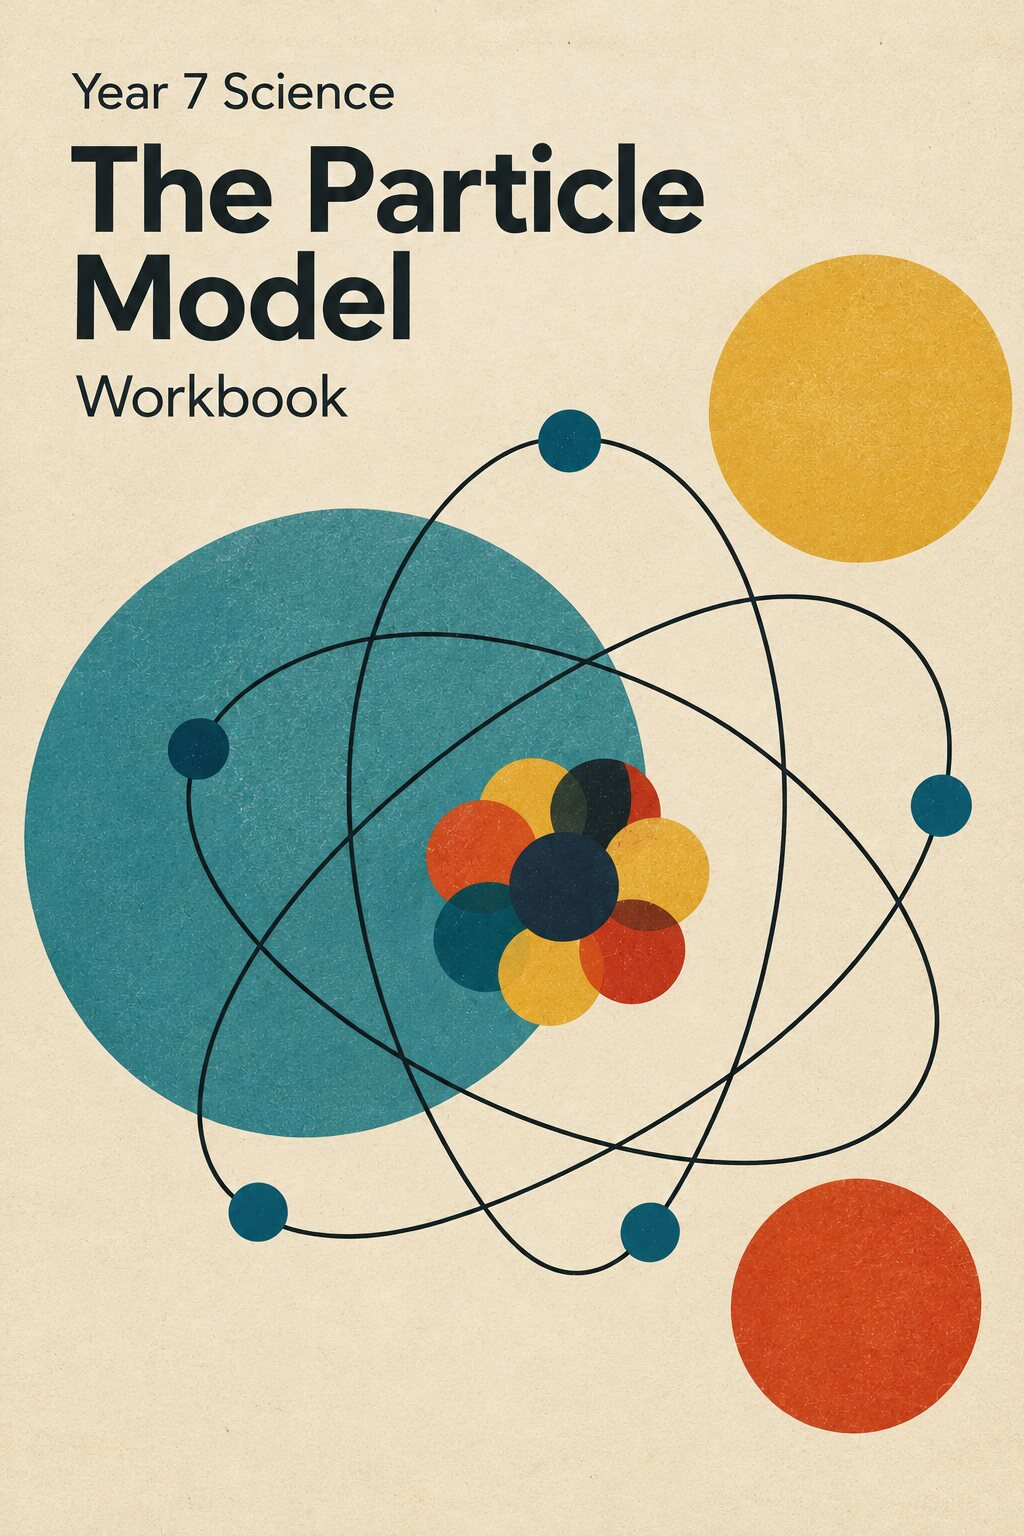
\includegraphics[width=\paperwidth]{../../covers/particle-model.jpg}};
  % Name box, top right, clear of the baked-in title ("The Particle" ends ~145 mm in).
  \node[anchor=north east, fill=white, draw=Ink, line width=0.6pt, rounded corners=1.5mm,
        inner xsep=2.6mm, inner ysep=2.2mm, text width=40mm, font=\headingfont\small]
    at ([xshift=-6mm, yshift=-6mm]current page.north east)
    {\textbf{Name}\par\vspace{5mm}\hrule\vspace{2.6mm}\textbf{Class}\par\vspace{5mm}\hrule};
  % What this book is: the cover art says Workbook, so name the booklet here.
  \node[anchor=south east, fill=white, draw=Ink, line width=0.6pt, rounded corners=1.5mm,
        inner xsep=3.2mm, inner ysep=2.4mm, font=\headingfont\bfseries\large, align=right]
    at ([xshift=-6mm, yshift=8mm]current page.south east)
    {Experiment Booklet\\[-1pt]{\normalfont\headingfont\small Mini-lab A \textbullet\ Experiments 1--3}};
\end{tikzpicture}
\mbox{}
\clearpage

% ---- Inside cover ---------------------------------------------------------
\thispagestyle{plain}
{\headingfont\bfseries\fontsize{26}{30}\selectfont The Particle Model}\par\vspace{1mm}
{\headingfont\Large Experiment Booklet \textbullet\ Year 7}\par\vspace{1mm}
{\small\itshape VC 2.0: VC2S8U05 \textbullet\ VC2S8I01--I08 \textbullet\ VC2S8H01}\par\vspace{6mm}
\renewcommand{\arraystretch}{2.2}
\begin{tabular}{@{}l p{130mm}@{}}
\textbf{Name} & \hrulefill \\ \textbf{Class} & \hrulefill \\ \textbf{Teacher} & \hrulefill \\ \textbf{Lab group} & \hrulefill \\
\end{tabular}
\renewcommand{\arraystretch}{1}

\begin{countrybox}{Acknowledgement of Country}
This booklet was created on the unceded Country of the Wurundjeri Woi-wurrung people of the Kulin Nation. We acknowledge Elders past, present and emerging. Aboriginal and Torres Strait Islander peoples have observed, tested and passed on knowledge of Country for tens of thousands of years: science in the way this booklet teaches it, by careful observation, measurement and sharing what was found.
\end{countrybox}

\begin{infobox}{How this booklet works}
This booklet holds every experiment in the unit. Bring it to every practical lesson. Each experiment opens with its key vocabulary, learning intentions and skills focus, then runs \emph{Technique} $\rightarrow$ \emph{Plan and safety} $\rightarrow$ \emph{Method} $\rightarrow$ \emph{Results} $\rightarrow$ \emph{Analysis and evaluation} $\rightarrow$ \emph{Skill check}. Each kind of box has its own frame and mark:\par\smallskip
\renewcommand{\arraystretch}{1.35}
\begin{tabular}{@{}p{32mm}l@{}}
\textbf{Technique} \tagicon{\icokey} & How to do it properly (thin frame) \\
\textbf{I do} \tagicon{\icodots{1}} & Your teacher works an example through --- you follow (solid frame) \\
\textbf{We do} \tagicon{\icodots{2}} & You try one together, with help (dashed frame) \\
\textbf{You do} \tagicon{\icodots{3}} & On your own: check your understanding (heavy frame) \\
\textbf{Going further} \tagicon{\icoup} & Above level: Year 8 extension (double frame) \\
\textbf{Skills focus} \tagicon{\icoskill} & The science skills the experiment builds \\
\end{tabular}

\smallskip
Every skill comes from the faculty \textbf{Science Skills} list (the toolkit on page \pageref{sec:toolkit}). A skill always carries the same code, for example \sk{PC4} or \sk{PA1}, so you can follow it from this unit into every other unit this year.
\end{infobox}

\clearpage
{\headingfont\bfseries\LARGE Contents}\par\vspace{1mm}\noindent\rule{\linewidth}{0.6pt}\par\vspace{2mm}
\begin{ctab}
\renewcommand{\arraystretch}{1.5}
\begin{tabular}{|L{2.8cm}|L{10.2cm}|C{1.6cm}|}
  \hline\thead{Section} & \thead{Title} & \thead{Page} \\ \hline
  Skills & \hyperlink{toolkit}{The Science Skills toolkit} & \hyperlink{toolkit}{\pageref{sec:toolkit}} \\ \hline
  Skills & \hyperlink{tracker}{My skills tracker} & \hyperlink{tracker}{\pageref{sec:tracker}} \\ \hline
  Mini-lab A & \hyperlink{exp.A}{The Viscosity Race (Lesson 1)} & \hyperlink{exp.A}{\pageref{sec:A}} \\ \hline
  Experiment 1 & \hyperlink{exp.1}{Matter Has Mass and Takes Up Space (Lesson 3)} & \hyperlink{exp.1}{\pageref{sec:1}} \\ \hline
  Experiment 2 & \hyperlink{exp.2}{A Cooling Curve (Lesson 6)} & \hyperlink{exp.2}{\pageref{sec:2}} \\ \hline
  Experiment 3 & \hyperlink{exp.3}{Density by Displacement (Lesson 9)} & \hyperlink{exp.3}{\pageref{sec:3}} \\ \hline
  Glossary & \hyperlink{glossary}{Key vocabulary, with the page each word first appears on} & \hyperlink{glossary}{\pageref{sec:glossary}} \\ \hline
\end{tabular}
\end{ctab}

% ══════════════════════════════════════════════════════════════════════════════
%  THE SCIENCE SKILLS TOOLKIT — faculty continuum, Years 7–8 column
% ══════════════════════════════════════════════════════════════════════════════
\clearpage
\hypertarget{toolkit}{}\pdfbookmark[1]{The Science Skills toolkit}{toolkitbm}
\markboth{The Science Skills toolkit}{}{\headingfont\bfseries\LARGE The Science Skills toolkit}\label{sec:toolkit}\par\vspace{1mm}\noindent\rule{\linewidth}{0.6pt}\par
These are the skills scientists use in every investigation. They come from the Science Inquiry strand of the Victorian Curriculum, grouped the way our faculty teaches them. Each experiment in this booklet tells you which skills it builds.

\newcommand{\tkhead}[2]{\multicolumn{3}{|l|}{\cellcolor{black!10}\rule{0pt}{4.6mm}\headingfont\bfseries #2} \\ \hline}
\newcommand{\tkrow}[1]{\skc{#1}\enspace{\small\bfseries\skname{#1}} & \skdesc{#1} & {\small\skcode{#1}} \\ \hline}
\renewcommand{\arraystretch}{1.35}
\begin{ctab}
\begin{longtable}{|W{5.0cm}|W{9.0cm}|Z{1.7cm}|}
  \hline\thead{Skill} & \thead{What it means} & \thead{Code} \\ \hline
  \endhead
  \tkhead{Teal}{Questioning and predicting}
  \tkrow{QP1}
  \tkrow{QP2}
  \tkhead{Blue}{Planning and conducting}
  \tkrow{PC1}
  \tkrow{PC2}
  \tkrow{PC3}
  \tkrow{PC4}
  \tkrow{PC5}
  \tkrow{PC6}
  \tkrow{PC7}
  \tkrow{PC8}
  \tkhead{GoldDark}{Processing, modelling and analysing}
  \tkrow{PA1}
  \tkrow{PA2}
  \tkrow{PA3}
  \tkrow{PA4}
  \tkrow{PA5}
  \tkrow{PA6}
  \tkrow{PA7}
  \tkrow{PA8}
  \tkhead{OrangeDark}{Evaluating}
  \tkrow{EV1}
  \tkrow{EV2}
  \tkrow{EV3}
  \tkrow{EV4}
  \tkrow{EV5}
  \tkhead{PurpleDark}{Communicating}
  \tkrow{CO1}
  \tkrow{CO2}
\end{longtable}
\end{ctab}
\renewcommand{\arraystretch}{1}

\begin{infobox}{Writing like a scientist \textbar\ CO1 \skname{CO1}}
Scientists write in the \textbf{third person}: say what was done, not who did it. Write \emph{``The water was heated for 10 minutes''}, not \emph{``I heated the water for 10 minutes''}. Keep sentences short, spell scientific words correctly, and always give a unit with a measurement.
\end{infobox}

% ══════════════════════════════════════════════════════════════════════════════
%  SKILLS TRACKER
% ══════════════════════════════════════════════════════════════════════════════
\clearpage
\hypertarget{tracker}{}\pdfbookmark[1]{My skills tracker}{trackerbm}
\markboth{My skills tracker}{}{\headingfont\bfseries\LARGE My skills tracker}\label{sec:tracker}\par\vspace{1mm}\noindent\rule{\linewidth}{0.6pt}\par
A dot \textbullet{} shows the experiments that build each skill. After each experiment, write how confident you are with each of its skills in its column: \textbf{1}~not yet, \textbf{2}~nearly, \textbf{3}~got it.

\newcommand{\dotc}{{\Large\textbullet}}
\newcommand{\trow}[5]{\rule[-0.36cm]{0pt}{0.92cm}\skc{#1}\enspace{\small\skname{#1}} & #2 & #3 & #4 & #5 & \\ \hline}
\begin{ctab}
\begin{tabular}{|W{5.4cm}|Z{1.5cm}|Z{1.5cm}|Z{1.5cm}|Z{1.5cm}|Z{2.2cm}|}
  \hline\thead{Skill} & \thead{Mini-lab A} & \thead{Exp 1} & \thead{Exp 2} & \thead{Exp 3} & \thead{End of unit} \\ \hline
  \trow{QP1}{\dotc}{\dotc}{\dotc}{\dotc}
  \trow{PC2}{\dotc}{}{}{}
  \trow{PC3}{}{}{\dotc}{}
  \trow{PC4}{}{\dotc}{}{\dotc}
  \trow{PC6}{\dotc}{\dotc}{\dotc}{}
  \trow{PC7}{}{}{}{\dotc}
  \trow{PC8}{\dotc}{}{}{}
  \trow{PA1}{\dotc}{\dotc}{}{\dotc}
  \trow{PA2}{}{}{\dotc}{}
  \trow{PA3}{\dotc}{\dotc}{}{\dotc}
  \trow{PA4}{}{}{\dotc}{}
  \trow{PA5}{\dotc}{}{\dotc}{}
  \trow{PA7}{}{}{\dotc}{}
  \trow{PA8}{}{}{\dotc}{}
  \trow{EV1}{\dotc}{\dotc}{\dotc}{\dotc}
  \trow{EV2}{}{}{\dotc}{\dotc}
  \trow{EV3}{}{\dotc}{\dotc}{\dotc}
  \trow{CO1}{}{}{}{\dotc}
\end{tabular}
\end{ctab}
{\small\color{DarkGrey} Skills not in this unit (QP2, PC1, PC5, PA6, EV4, EV5, CO2) are built in the experiment booklets for other units. Graphing \sk{PA2} starts here, in Experiment 2.}

% ══════════════════════════════════════════════════════════════════════════════
%  MINI-LAB A — THE VISCOSITY RACE                                     (Lesson 1)
%  A short class investigation inside Lesson 1, lettered so that Experiments
%  1–3 keep the numbers the decks and the lesson booklet already use.
% ══════════════════════════════════════════════════════════════════════════════
\renewcommand{\thesection}{A}\renewcommand{\symid}{0}
\renewcommand{\expword}{Mini-lab}\renewcommand{\expcaps}{MINI-LAB}
\experimentdiv{The Viscosity Race}{Planning a fair test \textbullet{} Timing with a stopwatch \textbullet{} Ranking liquids by how easily they flow}{1}\label{sec:A}
\lessoncodes{VC2S8U05 \textbullet{} VC2S8I01--I05}

\vocabhead
\begin{ctab}
\begin{tabular}{|SW{4.2cm}|W{11.6cm}|}
  \hline\hd & \thead{Word} & \thead{Definition (copy from the slide)} \\ \hline
  & \scaf{\textbf{Viscosity}\label{voc:viscosity}} & \scaf{How thick a liquid is: how much it resists flowing. Honey has a high viscosity.} \\ \hline
  & \textbf{Fair test}\label{voc:fair-test} & \\ \hline
  & \textbf{Variable}\label{voc:variable} & \\ \hline
  & \textbf{Trial}\label{voc:trial} & \\ \hline
  & \textbf{Average}\label{voc:average} & \\ \hline
\end{tabular}
\end{ctab}

\begin{lipanel}
\inquiryli{Plan a fair test, and time each liquid with a stopwatch.}
\understandli{Compare how easily liquids flow, and rank them by viscosity.}
\sctitle
\begin{itemize}[leftmargin=1.4em, itemsep=0pt, topsep=1pt]
  \item I can name the variables I keep the same to make the race a fair test.
  \item I can time each liquid three times and calculate an average.
  \item I can rank liquids from lowest to highest viscosity, using my results as evidence.
\end{itemize}
\end{lipanel}

\begin{skillsfocus}
\focus{QP1}{Predict the order the liquids will finish in, and say why.}
\focus{PC2}{Decide what to change, what to measure and what to keep the same.}
\focus{PC6}{Time three trials for each liquid and record them straight away.}
\focus{PC8}{Start and stop the stopwatch at the start and finish lines.}
\focus{PA1}{Record your times in a table with units in the headings.}
\focus{PA5}{Describe how race time relates to viscosity.}
\end{skillsfocus}

% ─── TECHNIQUE ────────────────────────────────────────────────────────────────
\exppart{Technique spotlight}{Blue}

\begin{technique}{Making a race a fair test}{PC2}
A test is \textbf{fair} when only one thing is different between the runs, so any difference in the results must come from that one thing.
\begin{itemize}[leftmargin=1.4em, itemsep=1pt, topsep=3pt]
  \item The \textbf{independent variable} is what you change on purpose: here, \emph{which liquid} races.
  \item The \textbf{dependent variable} is what you measure: here, \emph{the time to reach the finish line}.
  \item The \textbf{controlled variables} are everything you keep the same: the amount of liquid, the slope of the tile, the distance between the lines, the room temperature.
\end{itemize}
Run each liquid more than once. Each run is a \textbf{trial}; the average of three trials is more reliable than one.
\end{technique}

\begin{workedex}{Variables in a toy-car race}
Three toy cars are rolled down the same ramp to find which is fastest. Identify the variables.

\smallskip
\textbf{Independent:} which car is used. \quad \textbf{Dependent:} the time to reach the bottom.\\
\textbf{Controlled:} the same ramp, the same slope, the same starting line, and letting go without pushing.
\end{workedex}

\begin{wedo}{Variables in the viscosity race}
Complete the table for the viscosity race.
\begin{ctab}
\begin{tabular}{|SW{4.0cm}|W{10.6cm}|}
  \hline\hd & \thead{Variable} & \thead{In the viscosity race} \\ \hline
  & Independent & \\ \hline
  & Dependent & \\ \hline
  & Controlled (1) & \\ \hline
  & Controlled (2) & \\ \hline
\end{tabular}
\end{ctab}
\end{wedo}

\begin{technique}{Timing with a stopwatch}{PC8}
Share the jobs: one person \textbf{releases} the liquid, one \textbf{times}, one \textbf{records}. The timer starts the stopwatch the moment the front of the liquid crosses the start line, and stops it the moment it crosses the finish line. Record the time to one decimal place, in seconds (s). Reset the stopwatch before the next trial.
\end{technique}

\begin{youdobox}[Averages]
\task Calculate the average time for each liquid. Round to one decimal place. \skr{PA3}

\begin{ctab}
\begin{tabular}{|SW{3.4cm}|Z{2.3cm}|Z{2.3cm}|Z{2.3cm}|Z{3.6cm}|}
  \hline\hd & \thead{Liquid} & \thead{Trial 1 (s)} & \thead{Trial 2 (s)} & \thead{Trial 3 (s)} & \thead{Average (s)} \\ \hline
  & \scaf{e.g. milk} & \scaf{2.1} & \scaf{2.4} & \scaf{2.2} & \scaf{$6.7 \div 3 \approx 2.2$} \\ \hline
  & Shampoo & 18.2 & 17.6 & 18.4 & \\ \hline
  & Tomato sauce & 31.0 & 29.4 & 30.2 & \\ \hline
\end{tabular}
\end{ctab}
\end{youdobox}

% ─── PLAN AND SAFETY / METHOD ────────────────────────────────────────────────
\exppart{Plan, safety and method}{Teal}

\textbf{Aim:} To compare the viscosity of four liquids by timing how long each takes to run down a sloping tile.

\needspace{10\baselineskip}
\task Predict the order the four liquids will finish in, from fastest to slowest, and explain your prediction. The liquids are water, cooking oil, dishwashing liquid and honey. \skr{QP1}
\answerbox{5cm}

\subsubsection*{Equipment}
\begin{multicols}{2}
\begin{itemize}[leftmargin=1.2em, itemsep=0pt, topsep=0pt]
  \item smooth white tile (or plastic tray)
  \item two textbooks, to prop the tile up
  \item ruler and whiteboard marker
  \item four 5\,mL measuring spoons (one per liquid)
  \item water, cooking oil, dishwashing liquid, honey
  \item stopwatch
  \item paper towel
\end{itemize}
\end{multicols}

\begin{center}
\begin{tikzpicture}[scale=0.9]
  \draw[eq] (-0.2,0) -- (9.2,0);
  \draw[eq] (0,0) rectangle (2.0,0.55) (0.1,0.55) rectangle (1.9,1.1);
  \draw[eq] (0.3,1.25) -- (8.6,0.05) -- (8.5,-0.05) -- (0.25,1.1) -- cycle;
  \draw[Ink, line width=1.2pt] (1.95,1.03) -- (2.1,1.2);
  \draw[Ink, line width=1.2pt] (6.6,0.37) -- (6.75,0.55);
  \fill[black!70] (1.6,1.08) ellipse (0.16 and 0.07);
  \eqlab{(2.05,1.15)}{(2.3,2.2)}{start line}
  \eqlab{(6.7,0.5)}{(7.0,1.6)}{finish line, 20\,cm down the tile}
  \eqlabl{(1.0,0.85)}{(-0.3,2.0)}{textbooks}
  \eqlab{(4.5,0.65)}{(4.6,1.9)}{tile}
\end{tikzpicture}
\expfigcap{Scientific diagram of the viscosity race.}
\end{center}

\begin{infobox}{Safety}
Spilt oil, honey and dishwashing liquid make the bench and floor slippery: wipe spills up straight away. Never taste anything in the lab. Wash your hands at the end.
\end{infobox}

\subsubsection*{Method}
\begin{enumerate}[itemsep=2pt]
  \item Prop one end of the tile on two textbooks. Draw a start line near the top and a finish line 20\,cm further down.
  \item Fill a measuring spoon level with the first liquid.
  \item Pour the liquid just above the start line. The timer starts the stopwatch as the front of the liquid crosses the start line.
  \item Stop the stopwatch as the front of the liquid crosses the finish line. Record the time.
  \item Wipe the tile clean and dry. Repeat for two more trials.
  \item Repeat steps 2--5 for each of the other liquids, keeping the tile at the same slope.
\end{enumerate}

% ─── RESULTS ─────────────────────────────────────────────────────────────────
\exppart{Results}{Amber}

\subsubsection*{Time for each liquid to run 20\,cm down the tile \skr{PA1}}
\begin{ctab}
\begin{tabular}{|SW{3.4cm}|Z{2.1cm}|Z{2.1cm}|Z{2.1cm}|Z{2.6cm}|Z{2.2cm}|}
  \hline\hd & \thead{Liquid} & \thead{Trial 1 (s)} & \thead{Trial 2 (s)} & \thead{Trial 3 (s)} & \thead{Average (s)} & \thead{Rank (1 = fastest)} \\ \hline
  & \scaf{e.g. milk} & \scaf{2.1} & \scaf{2.4} & \scaf{2.2} & \scaf{2.2} & \scaf{---} \\ \hline
  & Water & & & & & \\ \hline
  & Cooking oil & & & & & \\ \hline
  & Dishwashing liquid & & & & & \\ \hline
  & Honey & & & & & \\ \hline
\end{tabular}
\end{ctab}

\needspace{10\baselineskip}
\task Write down anything you observed while the liquids ran, other than the times (for example, the shape of the liquid or how it spread).
\answerbox{5cm}

% ─── ANALYSIS ────────────────────────────────────────────────────────────────
\exppart{Analysis and evaluation}{Coral}

\task List the four liquids from lowest viscosity to highest viscosity. \skr{PA5}
\answerbox{1.2cm}

\needspace{10\baselineskip}
\task Describe the relationship between a liquid's race time and its viscosity. Use two liquids from your results as evidence. \skr{PA5}

\scaf{The longer a liquid took to reach the finish line, the \dots. For example, \dots\ took \dots\,s but \dots\ took \dots\,s.}
\answerbox{5cm}

\needspace{10\baselineskip}
\task Was your prediction correct? Use your results to explain. \skr{EV1}
\answerbox{5cm}

\needspace{10\baselineskip}
\task Explain why each liquid was timed three times instead of once. \skr{PC6}
\answerbox{5cm}

\needspace{14\baselineskip}
\task A group used a full spoon of honey but only half a spoon of water. \skr{PC2}
\pt{a}Which controlled variable did they change?
\answerbox{1cm}
\pt{b}Explain why this makes their race unfair.
\answerbox{5cm}

\begin{yr8box}
\begin{keepext}
\exttask Honey flows much more easily when it is warm. Predict how the honey's race time would change if the honey and the tile were warmed to 40\,\textdegree C, and design a fair test to check your prediction.
\answerbox{5cm}
\end{keepext}
\begin{keepext}
\exttask Toothpaste does not flow down the tile at all unless it is pushed, but it is not a solid either. Suggest how you could decide whether toothpaste is a solid or a liquid.
\answerbox{5cm}
\end{keepext}
\end{yr8box}

% ─── SKILL CHECK ─────────────────────────────────────────────────────────────
\exppart{Skill check}{NavyBlue}

\begin{skillcheck}
\scrow{QP1}{I can predict an order and give a reason for my prediction.}
\scrow{PC2}{I can name the variables I change, measure and keep the same in a fair test.}
\scrow{PC6}{I timed three trials for each liquid and recorded them straight away.}
\scrow{PC8}{I started and stopped the stopwatch at the lines.}
\scrow{PA1}{I recorded my results in a table with units in the headings.}
\scrow{PA5}{I can describe how race time relates to viscosity, using data.}
\end{skillcheck}

\task Which skill will you focus on in Experiment 1? Explain what you will do differently.
\answerbox{5cm}

% back to numbered experiments
\setcounter{section}{0}\renewcommand{\thesection}{\arabic{section}}\renewcommand{\symid}{\thesection}
\renewcommand{\expword}{Experiment}\renewcommand{\expcaps}{EXPERIMENT}
% ══════════════════════════════════════════════════════════════════════════════
%  EXPERIMENT 1 — MATTER HAS MASS AND TAKES UP SPACE                   (Lesson 3)
%  Content from the lesson booklet's Lesson 3, plus the dry ice demonstration
%  from the unit plan.
% ══════════════════════════════════════════════════════════════════════════════
\experimentdiv{Matter Has Mass and Takes Up Space}{Dry ice demonstration \textbullet{} Does air have mass? \textbullet{} Does air take up space?}{3}\label{sec:1}
\lessoncodes{VC2S8U05 \textbullet{} VC2S8I01, I02, I04, I06}

\vocabhead
\begin{ctab}
\begin{tabular}{|SW{4.2cm}|W{11.6cm}|}
  \hline\hd & \thead{Word} & \thead{Definition (copy from the slide)} \\ \hline
  & \scaf{\textbf{Matter}\label{voc:matter}} & \scaf{Anything that has mass and takes up space.} \\ \hline
  & \textbf{Observation}\label{voc:observation} & \\ \hline
  & \textbf{Inference}\label{voc:inference} & \\ \hline
  & \textbf{Sublimation}\label{voc:sublimation} & \\ \hline
  & \textbf{Tare}\label{voc:tare} & \\ \hline
\end{tabular}
\end{ctab}

\begin{lipanel}
\inquiryli{Use a balance to take precise readings, and record them in a table.}
\understandli{Explain, with evidence, that gases are matter: they have mass and take up space.}
\sctitle
\begin{itemize}[leftmargin=1.4em, itemsep=0pt, topsep=1pt]
  \item I can tell an observation from an inference.
  \item I can measure a small change in mass and calculate the difference and the average.
  \item I can use my results to explain that air has mass and takes up space.
\end{itemize}
\end{lipanel}

\begin{skillsfocus}
\focus{QP1}{Predict what will happen to the ball's mass, and why.}
\focus{PC4}{Use the same balance, tared, and keep every decimal place.}
\focus{PC6}{Record observations of the demonstration and both tests.}
\focus{PA1}{Record masses in a table with units in the headings.}
\focus{PA3}{Calculate each increase in mass, and the average increase.}
\focus{EV1}{Say whether your results support your prediction.}
\focus{EV3}{Name what could make the mass readings less accurate.}
\end{skillsfocus}

% ─── TECHNIQUE ────────────────────────────────────────────────────────────────
\exppart{Technique spotlight}{Blue}

\begin{technique}{Observation or inference?}{PC6}
An \textbf{observation} is what you can see, hear, feel or measure: \emph{the balloon got bigger}. An \textbf{inference} is an explanation of an observation: \emph{gas came off the dry ice and filled the balloon}. Record observations first. Keep inferences for the analysis, and back each one with an observation.
\end{technique}

\begin{workedex}{Sorting statements}
A teacher drops dry ice into warm water. Sort the statements.

\smallskip
\begin{tabular}{@{}p{9.4cm}l@{}}
\emph{White fog spills over the side of the beaker.} & \textbf{Observation} --- it can be seen. \\
\emph{The water is bubbling.} & \textbf{Observation} --- it can be seen and heard. \\
\emph{The bubbles are carbon dioxide gas.} & \textbf{Inference} --- it explains what is seen. \\
\end{tabular}
\end{workedex}

\begin{wedo}{Sorting statements}
Write \emph{observation} or \emph{inference} for each statement.
\begin{ctab}
\begin{tabular}{|SW{10.4cm}|W{4.6cm}|}
  \hline\hd & \thead{Statement} & \thead{Observation or inference?} \\ \hline
  & The piece of dry ice is getting smaller. & \\ \hline
  & The dry ice is turning straight into a gas. & \\ \hline
  & The balloon on the flask inflated. & \\ \hline
\end{tabular}
\end{ctab}
\end{wedo}

\begin{technique}{Measuring a small change in mass}{PC4}
Pumping air into a ball changes its mass by only a few grams, so every reading has to be as precise as possible.
\begin{enumerate}[leftmargin=1.6em, itemsep=1pt, topsep=3pt]
  \item Use the \textbf{same} balance for the before and after readings.
  \item Check it reads 0.00\,g with nothing on it, and keep every decimal place.
  \item Find the change \textbf{by difference}: mass after $-$ mass before.
  \item Repeat the test three times and average the changes.
\end{enumerate}
\end{technique}

\begin{workedex}{Mass by difference}
A student forgets to tare the balance. An empty beaker reads 52.40\,g. With salt in it, it reads 67.15\,g. What is the mass of the salt?

\medskip
\textbf{Mass of salt} = mass with salt $-$ mass of empty beaker $= 67.15 - 52.40 = \mathbf{14.75\ g}$
\end{workedex}

\begin{wedo}{Mass by difference}
An empty plastic cup has a mass of 8.30\,g. Filled with sand, it has a mass of 126.80\,g. What is the mass of the sand?
\workbox{3cm}
\end{wedo}

\begin{youdobox}[Changes in mass]
\taskpair{A ball had a mass of 410.50\,g before pumping and 413.10\,g after. Find the mass of air added.}{3.0cm}
         {Three tests added 2.60\,g, 2.75\,g and 2.65\,g of air. Find the average mass of air added.}{3.0cm}
\end{youdobox}

% ─── PLAN AND SAFETY / METHOD ────────────────────────────────────────────────
\exppart{Plan, safety and method}{Teal}

\textbf{Aim:} To show that air has mass and takes up space.

\needspace{10\baselineskip}
\task Will a ball weigh more, less or the same after you pump more air into it? Write your prediction and explain it. \skr{QP1}
\answerbox{5cm}

\subsubsection*{Equipment}
\begin{multicols}{2}
\begin{itemize}[leftmargin=1.2em, itemsep=0pt, topsep=0pt]
  \item soft ball with a valve (basketball or netball)
  \item ball pump with a needle
  \item electronic balance (reads to 0.01\,g)
  \item large clear tub of water
  \item clear plastic cup
  \item paper towel and sticky tape
\end{itemize}
\end{multicols}

\begin{infobox}{Safety}
\textbf{Demonstration:} only your teacher handles dry ice. At $-78$\,\textdegree C it burns skin on contact, and it is never sealed in a closed container. Watch from where your teacher tells you to stand.\par
\textbf{Your tests:} wipe up spilt water straight away --- a wet floor is a slip hazard. Keep the pump needle pointed away from people, and keep water away from the balance and its power cord.
\end{infobox}

\subsubsection*{Demonstration --- Dry ice (your teacher)}
Your teacher puts a piece of dry ice (solid carbon dioxide) on the bench, drops some into warm water, and puts some in a flask with a balloon stretched over its neck. Record what you observe in Table 1.1.

\subsubsection*{Method --- Part 1: Does air have mass?}
\begin{enumerate}[itemsep=2pt]
  \item Let some air out of the ball so it is soft but still round.
  \item Check the balance reads 0.00\,g, put the ball on it, and record its mass.
  \item Pump the ball until it is firm. Count the number of pumps.
  \item Weigh the ball again and record its mass.
  \item Repeat the whole test two more times.
\end{enumerate}

\subsubsection*{Method --- Part 2: Does air take up space?}
\begin{enumerate}[itemsep=2pt]
  \item Scrunch a paper towel and tape it into the bottom of the cup so it cannot fall out.
  \item Turn the cup upside down and push it straight down to the bottom of the tub. Do not tilt it.
  \item Lift it straight out, and feel the paper towel.
  \item Now repeat, but tilt the cup while it is under water. Watch what comes out.
\end{enumerate}

% ─── RESULTS ─────────────────────────────────────────────────────────────────
\exppart{Results}{Amber}

\subsubsection*{Table 1.1 --- Dry ice demonstration \skr{PC6}}
\begin{ctab}
\begin{tabular}{|SW{3.4cm}|W{5.8cm}|W{5.8cm}|}
  \hline\hd & \thead{Dry ice \dots} & \thead{What I observed} & \thead{What I infer from it} \\ \hline
  & \scaf{e.g. held over a candle flame} & \scaf{The flame went out.} & \scaf{The gas does not let things burn.} \\ \hline
  & on the bench & & \\ \hline
  & in warm water & & \\ \hline
  & in a flask with a balloon & & \\ \hline
\end{tabular}
\end{ctab}

\subsubsection*{Table 1.2 --- Does air have mass? \skr{PA1}}
\begin{ctab}
\begin{tabular}{|SZ{1.6cm}|Z{3.3cm}|Z{2.0cm}|Z{3.3cm}|Z{4.4cm}|}
  \hline\hd & \thead{Test} & \thead{Mass before pumping (g)} & \thead{Pumps} & \thead{Mass after pumping (g)} & \thead{Increase in mass (g)} \\ \hline
  & \scaf{e.g.} & \scaf{598.20} & \scaf{20} & \scaf{601.65} & \scaf{$601.65 - 598.20 = 3.45$} \\ \hline
  & 1 & & & & \\ \hline
  & 2 & & & & \\ \hline
  & 3 & & & & \\ \hline
  \multicolumn{5}{|r|}{\rule{0pt}{1.5cm}\headingfont\bfseries Average increase in mass (g)} & \\ \hline
\end{tabular}
\end{ctab}

\subsubsection*{Table 1.3 --- Does air take up space?}
\begin{ctab}
\begin{tabular}{|SW{5.0cm}|W{10.0cm}|}
  \hline\hd & \thead{Test} & \thead{What I observed} \\ \hline
  & \scaf{e.g. an empty cup pushed down} & \scaf{The water only came part of the way up inside the cup.} \\ \hline
  & Cup pushed straight down: the paper towel & \\ \hline
  & Cup tilted under water & \\ \hline
\end{tabular}
\end{ctab}

% ─── ANALYSIS ────────────────────────────────────────────────────────────────
\exppart{Analysis and evaluation}{Coral}

\task Did the ball's mass go up, go down, or stay the same when air was pumped in? Was your prediction correct? \skr{EV1}
\answerbox{5cm}

\needspace{10\baselineskip}
\task Explain what your results from Table 1.2 show about air. Use the word \emph{mass}.
\answerbox{5cm}

\needspace{10\baselineskip}
\task Explain why the paper towel stayed dry. Use the words \emph{air} and \emph{space}.
\answerbox{5cm}

\needspace{10\baselineskip}
\task What came out of the cup when you tilted it under water, and what does this show?
\answerbox{5cm}

\needspace{10\baselineskip}
\task The balloon on the flask inflated even though nothing was blown into it. Use the dry ice demonstration to explain where the gas came from, and what this shows about gases.
\answerbox{5cm}

\needspace{14\baselineskip}
\task Evaluate the method for Part 1. \skr{EV3}
\pt{a}Why did you repeat the ball test three times?
\answerbox{5cm}
\pt{b}Identify one thing that could have made your mass readings less accurate.
\answerbox{5cm}
\pt{c}Suggest one improvement to Part 1.
\answerbox{5cm}

\begin{yr8box}
\begin{keepext}
\exttask One litre of air has a mass of about 1.2\,g. A ball gained 3.6\,g when it was pumped up.
\pt{a}About how many litres of extra air were pushed into the ball?
\workbox{3cm}
\pt{b}The ball itself holds only about 7 litres. Explain how it can hold that much extra air.
\answerbox{5cm}
\end{keepext}
\begin{keepext}
\exttask A classroom is 8\,m long, 7\,m wide and 3\,m high. One cubic metre of air has a mass of about 1.2\,kg. Calculate the volume of the room and the mass of air in it.
\workbox{4cm}
\end{keepext}
\begin{keepext}
\exttask A student weighs a balloon before and after blowing it up and finds almost no change. She concludes that air has no mass. Suggest why her result might have been misleading, and how Part 1 of your experiment avoided the problem.
\answerbox{5cm}
\end{keepext}
\end{yr8box}

% ─── SKILL CHECK ─────────────────────────────────────────────────────────────
\exppart{Skill check}{NavyBlue}

\begin{skillcheck}
\scrow{QP1}{I can write a prediction and explain it.}
\scrow{PC4}{I used the same balance, checked it read zero, and kept every decimal place.}
\scrow{PC6}{I can record observations, and tell them apart from inferences.}
\scrow{PA1}{I recorded masses in a table with units in the headings.}
\scrow{PA3}{I can calculate a change in mass by difference, and an average.}
\scrow{EV1}{I can say whether my results supported my prediction.}
\scrow{EV3}{I can name what could make a reading less accurate, and suggest an improvement.}
\end{skillcheck}

\task Which skill will you focus on in Experiment 2? Explain what you will do differently.
\answerbox{5cm}
% ══════════════════════════════════════════════════════════════════════════════
%  EXPERIMENT 2 — A COOLING CURVE                                       (Lesson 6)
%  Content from the A4 master's Lesson 9. First line graph of the year.
% ══════════════════════════════════════════════════════════════════════════════
\experimentdiv{A Cooling Curve}{Temperature over time \textbullet{} Line graphs \textbullet{} The freezing point \textbullet{} The plateau}{6}\label{sec:2}
\lessoncodes{VC2S8U05 \textbullet{} VC2S8I01--I06}

\vocabhead
\begin{ctab}
\begin{tabular}{|SW{4.2cm}|W{11.6cm}|}
  \hline\hd & \thead{Word} & \thead{Definition (copy from the slide)} \\ \hline
  & \scaf{\textbf{Cooling curve}\label{voc:cooling-curve}} & \scaf{A line graph showing how the temperature of a substance falls over time.} \\ \hline
  & \textbf{Freezing point}\label{voc:freezing-point} & \\ \hline
  & \textbf{Line graph}\label{voc:line-graph} & \\ \hline
  & \textbf{Axis}\label{voc:axis} & \\ \hline
  & \textbf{Plateau}\label{voc:plateau} & \\ \hline
\end{tabular}
\end{ctab}

\begin{lipanel}
\inquiryli{Record temperature every minute, then draw a line graph and describe the pattern.}
\understandli{Find the freezing point from the graph, and explain why the temperature stays constant while a substance freezes.}
\sctitle
\begin{itemize}[leftmargin=1.4em, itemsep=0pt, topsep=1pt]
  \item I can record the temperature every minute and draw a line graph with labelled axes, even scales and a title.
  \item I can read the freezing point from my graph and explain the plateau using particles.
\end{itemize}
\end{lipanel}

\begin{skillsfocus}
\focus{QP1}{Sketch how the temperature will change.}
\focus{PC3}{Assess the risks before you start.}
\focus{PC6}{Read the temperature every minute.}
\focus{PA2}{Draw your first line graph.}
\focus{PA5}{Describe the curve's shape.}
\focus{PA8}{Explain the plateau with particles.}
\focus{EV2}{Compare with the accepted 44\,\textdegree C.}
\end{skillsfocus}

% ─── TECHNIQUE ────────────────────────────────────────────────────────────────
\exppart{Technique spotlight}{Blue}

\begin{technique}{Drawing a line graph}{PA2}
\begin{minipage}[c]{0.56\linewidth}
\begin{enumerate}[leftmargin=1.6em, itemsep=1pt, topsep=0pt]
  \item Put the thing you \textbf{changed or controlled} (time) on the horizontal axis.
  \item Put the thing you \textbf{measured} (temperature) on the vertical axis.
  \item Choose an \textbf{even scale} for each axis that uses most of the grid.
  \item \textbf{Label} both axes with the quantity and the unit, e.g.\ \emph{time (minutes)}.
  \item \textbf{Plot} each point with a small cross, join the points with a smooth line, and give the graph a \textbf{title}.
\end{enumerate}
\end{minipage}\hfill
\begin{minipage}[c]{0.4\linewidth}\centering
\begin{tikzpicture}[x=0.5cm, y=0.05cm, font=\scriptsize]
  \foreach \m in {0,...,8}{\draw[black!25] (\m,20) -- (\m,70);}
  \foreach \t in {20,30,...,70}{\draw[black!25] (0,\t) -- (8,\t); \node[anchor=east] at (0,\t) {\t};}
  \foreach \m in {0,2,...,8}{\node[anchor=north] at (\m,20) {\m};}
  \draw[axis] (0,20) -- (8.5,20); \draw[axis] (0,20) -- (0,74);
  \draw[Ink, line width=1.2pt] plot[smooth] coordinates {(0,66) (1,55) (2,48) (3,44) (4,44) (5,44) (6,44) (7,40) (8,36)};
  \foreach \p in {(0,66),(1,55),(2,48),(3,44),(4,44),(5,44),(6,44),(7,40),(8,36)} \node[font=\small] at \p {$\times$};
  \node[anchor=north] at (4,13) {time (minutes)};
  \node[rotate=90, anchor=south] at (-1.1,45) {temperature (\textdegree C)};
\end{tikzpicture}
\end{minipage}
\end{technique}

\begin{workedex}{Choosing a scale}
Temperatures in a set of results go from 22\,\textdegree C up to 68\,\textdegree C. The grid has 15 big squares going up. Choose a scale for the temperature axis.

\medskip
Start just below the smallest value, at \textbf{20\,\textdegree C}. Going up in steps of \textbf{5\,\textdegree C} per big square, 15 squares reach $20 + 15 \times 5 = 95$\,\textdegree C. That fits every result and uses most of the grid.
\end{workedex}

\begin{wedo}{Choosing a scale}
Times in a set of results go from 0 to 12 minutes. The grid has 15 big squares going across. Choose a scale for the time axis, and show it fits.
\workbox{3cm}
\end{wedo}

\begin{youdobox}[Your first line graph]
\task A student heated 150\,mL of water and recorded its temperature every minute. Draw a line graph of the results. Label both axes with units and give the graph a title. \skr{PA2}

\begin{ctab}
\begin{tabular}{|l|*{11}{C{0.78cm}|}}
  \hline\thead{Time (min)} & 0 & 1 & 2 & 3 & 4 & 5 & 6 & 7 & 8 & 9 & 10 \\ \hline
  \thead{Temperature (\textdegree C)} & 18 & 27 & 36 & 45 & 53 & 61 & 69 & 77 & 84 & 91 & 97 \\ \hline
\end{tabular}
\end{ctab}
\graphgrid{15cm}
\end{youdobox}

% ─── PLAN AND SAFETY ─────────────────────────────────────────────────────────
\exppart{Plan and safety}{Teal}

\textbf{Aim:} To measure the temperature of lauric acid as it cools and freezes, and find its freezing point.

\begin{infobox}{Why lauric acid?}
Water would need a freezer to freeze. Lauric acid, a white waxy solid found in coconut oil, melts at a temperature hot water from a kettle can reach, so you can melt it and then watch it cool and freeze on the bench.
\end{infobox}

\needspace{14\baselineskip}
\task Sketch what you think the temperature of the lauric acid will do as it cools, then explain your sketch. Will it fall steadily the whole time? \skr{QP1}

\noindent\begin{minipage}[t]{0.42\linewidth}\drawbox{5cm}{\scriptsize temperature $\uparrow$ \hfill time $\rightarrow$}\end{minipage}\hfill
\begin{minipage}[t]{0.55\linewidth}\answerbox{5cm}\end{minipage}

\needspace{14\baselineskip}
\task Complete the risk assessment before you start. Your teacher must initial it. \skr{PC3}\par\nobreak\hfill\textbf{Teacher's initials:}\ \underline{\hspace{3cm}}
\begin{ctab}
\begin{tabular}{|SW{3.6cm}|W{4.6cm}|W{7.0cm}|}
  \hline\hd & \thead{Hazard} & \thead{Risk (what could happen)} & \thead{Control (how we prevent it)} \\ \hline
  & \scaf{Hot-water bath} & \scaf{Scalds to the hands} & \scaf{Collect the boiling tube with a test-tube holder, never with fingers.} \\ \hline
  & Lauric acid & & \\ \hline
  & Glass thermometer & & \\ \hline
  & Hot boiling tube & & \\ \hline
\end{tabular}
\end{ctab}

% ─── METHOD ──────────────────────────────────────────────────────────────────
\exppart{Method}{Teal}

\subsubsection*{Equipment}
\begin{multicols}{2}
\begin{itemize}[leftmargin=1.2em, itemsep=0pt, topsep=0pt]
  \item boiling tube of lauric acid, melted by your teacher in a hot-water bath
  \item test-tube holder
  \item thermometer ($-10$ to 110\,\textdegree C)
  \item retort stand and clamp
  \item 250\,mL beaker (empty)
  \item stopwatch
  \item safety glasses
\end{itemize}
\end{multicols}

\begin{center}
\begin{tikzpicture}[scale=0.95]
  \begin{scope}\eqStand\end{scope}
  \draw[eq] (2.2,0.2) -- (2.2,0.21);
  \draw[eq] (1.55,2.25) -- (1.55,0.6) arc[start angle=180,end angle=360,radius=0.3] -- (2.15,2.25);
  \fill[black!12] (1.57,1.5) -- (1.57,0.6) arc[start angle=180,end angle=360,radius=0.28] -- (2.13,1.5) -- cycle;
  \draw[Ink, line width=0.6pt] (1.57,1.5) -- (2.13,1.5);
  \draw[eq] (1.05,2.05) -- (1.25,1.9) -- (1.25,0.2) -- (2.45,0.2) -- (2.45,1.95);
  \draw[eq] (1.85,0.65) circle (0.1);
  \draw[eq] (1.79,0.74) -- (1.79,4.3) (1.91,0.74) -- (1.91,4.3);
  \eqlab{(1.91,3.9)}{(3.4,3.9)}{thermometer}
  \eqlab{(1.95,3.0)}{(3.4,3.2)}{clamp}
  \eqlab{(2.15,2.0)}{(3.4,2.4)}{boiling tube}
  \eqlab{(2.13,1.2)}{(3.4,1.6)}{lauric acid}
  \eqlab{(2.45,0.9)}{(3.4,0.8)}{empty beaker}
  \eqlabl{(0.35,3.6)}{(-0.4,3.6)}{retort stand}
\end{tikzpicture}
\expfigcap{Scientific diagram of the cooling curve set-up.}
\end{center}

\begin{enumerate}[itemsep=2pt]
  \item Put on safety glasses. Collect a boiling tube of melted lauric acid from the hot-water bath, using a test-tube holder.
  \item Clamp the boiling tube so it stands upright inside the empty beaker.
  \item Put the thermometer in the lauric acid, with its bulb in the middle of the liquid.
  \item When the temperature reads 65\,\textdegree C or just below, start the stopwatch and record the temperature.
  \item Record the temperature every minute for 12 minutes. Stir gently with the thermometer while the lauric acid is still liquid.
  \item Write down the time when you first see solid forming, and when it has all gone solid.
  \item Do not try to pull the thermometer out once the lauric acid is solid. Return the tube to the hot-water bath to melt it again.
\end{enumerate}

% ─── RESULTS ─────────────────────────────────────────────────────────────────
\exppart{Results}{Amber}

\subsubsection*{The temperature of lauric acid as it cools \skr{PC6}}
\begin{ctab}
\begin{tabular}{|SZ{3.2cm}|Z{3.6cm}|Z{3.2cm}|Z{3.6cm}|}
  \hline\hd & \thead{Time (min)} & \thead{Temperature (\textdegree C)} & \thead{Time (min)} & \thead{Temperature (\textdegree C)} \\ \hline
  & \scaf{e.g. 0} & \scaf{65} & \scaf{e.g. 7} & \scaf{44} \\ \hline
  & 0 & & 7 & \\ \hline
  & 1 & & 8 & \\ \hline
  & 2 & & 9 & \\ \hline
  & 3 & & 10 & \\ \hline
  & 4 & & 11 & \\ \hline
  & 5 & & 12 & \\ \hline
  & 6 & & & \\ \hline
\end{tabular}
\end{ctab}

\noindent Solid first seen at \rule{2.2cm}{0.4pt} minutes. \qquad All solid at \rule{2.2cm}{0.4pt} minutes.

\clearpage
\task Draw a cooling curve of your results. Put \textbf{time (minutes)} on the horizontal axis and \textbf{temperature (\textdegree C)} on the vertical axis. Plot each point, join them with a smooth line, and give the graph a title. \skr{PA2}

\vspace{3pt}
\graphgrid{16cm}

% ─── ANALYSIS ────────────────────────────────────────────────────────────────
\exppart{Analysis and evaluation}{Coral}

\task Describe the shape of your cooling curve, from start to finish. \skr{PA5}
\answerbox{5cm}

\needspace{14\baselineskip}
\task Use your graph. \skr{EV2}
\pt{a}Read the freezing point of lauric acid from your graph.
\answerbox{1cm}
\pt{b}The accepted freezing point of lauric acid is 44\,\textdegree C. Compare your value with it, and suggest one reason for any difference.
\answerbox{5cm}
\pt{c}For how many minutes did the temperature stay on the plateau?
\workbox{2cm}

\needspace{10\baselineskip}
\task Was your prediction correct? Explain, using your graph. \skr{EV1}
\answerbox{5cm}

\needspace{14\baselineskip}
\task Draw particle diagrams of the lauric acid before, during and after the plateau. Use the same number of particles, the same size, in each. \skr{PA4}

\noindent
\begin{minipage}[t]{0.32\linewidth}\centering\drawbox{4.5cm}{}{\small Before: liquid}\end{minipage}\hfill
\begin{minipage}[t]{0.32\linewidth}\centering\drawbox{4.5cm}{}{\small During: freezing}\end{minipage}\hfill
\begin{minipage}[t]{0.32\linewidth}\centering\drawbox{4.5cm}{}{\small After: solid}\end{minipage}

\needspace{10\baselineskip}
\task Explain, using particles, what was happening to the lauric acid during the plateau, and why the temperature stayed steady. \skr{PA8}
\answerbox{5cm}

\needspace{16\baselineskip}
\task Another group recorded these temperatures every minute, starting at 0 minutes: 64, 57, 51, 54, 44, 44, 44, 44, 43, 40, 37\,\textdegree C. \skr{PA7}
\pt{a}Which reading does not fit the pattern?
\answerbox{1cm}
\pt{b}Suggest what might have caused it.
\answerbox{5cm}
\pt{c}What freezing point do their results show?
\answerbox{1cm}

\needspace{14\baselineskip}
\task Evaluate the method. \skr{EV3}
\pt{a}Identify one source of error in this experiment.
\answerbox{5cm}
\pt{b}Suggest one way to make the results more reliable.
\answerbox{5cm}

\begin{yr8box}
\begin{keepext}
\exttask A group used twice as much lauric acid in their tube. Predict how their cooling curve would be different from yours, and how it would be the same. Explain both.
\answerbox{5cm}
\end{keepext}
\begin{keepext}
\exttask Candle wax is a mixture, not a pure substance. Its cooling curve has no flat plateau, only a part where the line slopes more gently. Suggest why.
\answerbox{5cm}
\end{keepext}
\begin{keepext}
\exttask The lauric acid cooled quickly at the start and slowly near the end. Think about how far its temperature was above room temperature in each case, and suggest a rule for how fast hot things cool.
\answerbox{5cm}
\end{keepext}
\end{yr8box}

% ─── SKILL CHECK ─────────────────────────────────────────────────────────────
\exppart{Skill check}{NavyBlue}

\begin{skillcheck}
\scrow{QP1}{I can sketch and explain a prediction.}
\scrow{PC3}{I completed a risk assessment and followed it.}
\scrow{PC6}{I recorded a reading at every whole minute, with its unit.}
\scrow{PA2}{I can draw a line graph with labelled axes, even scales, plotted points and a title.}
\scrow{PA5}{I can describe the shape of a cooling curve.}
\scrow{PA8}{I can use the particle model to explain the plateau.}
\scrow{EV2}{I can compare my result with the accepted value.}
\end{skillcheck}

\task Which skill will you focus on in Experiment 3? Explain what you will do differently.
\answerbox{5cm}
% ══════════════════════════════════════════════════════════════════════════════
%  EXPERIMENT 3 — DENSITY BY DISPLACEMENT                              (Lesson 9)
%  Content from the A4 master's Lesson 15.
% ══════════════════════════════════════════════════════════════════════════════
\experimentdiv{Density by Displacement}{Volume of an irregular object \textbullet{} Measuring mass and volume \textbullet{} Calculating density \textbullet{} Identifying the material}{9}\label{sec:3}
\lessoncodes{VC2S8U05 \textbullet{} VC2S8I01, I03, I04, I06, I08}

\vocabhead
\begin{ctab}
\begin{tabular}{|SW{4.2cm}|W{11.6cm}|}
  \hline\hd & \thead{Word} & \thead{Definition (copy from the slide)} \\ \hline
  & \scaf{\textbf{Displacement}\label{voc:displacement}} & \scaf{Water being pushed out of the way when an object is put into it.} \\ \hline
  & \textbf{Irregular object}\label{voc:irregular-object} & \\ \hline
  & \textbf{Density}\label{voc:density} & \\ \hline
  & \textbf{Accuracy}\label{voc:accuracy} & \\ \hline
  & \textbf{Conclusion}\label{voc:conclusion} & \\ \hline
\end{tabular}
\end{ctab}

\begin{lipanel}
\inquiryli{Measure volume by displacement and mass on a balance; process the data to calculate density.}
\understandli{Use density to identify a material and predict whether it floats.}
\sctitle
\begin{itemize}[leftmargin=1.4em, itemsep=0pt, topsep=1pt]
  \item I can find the volume of an irregular object by displacement.
  \item I can calculate density with $D = m \div V$ and the correct unit.
  \item I can use density to identify a material, and write a conclusion that answers the aim.
\end{itemize}
\end{lipanel}

\begin{skillsfocus}
\focus{QP1}{Predict the densest object.}
\focus{PC4}{Read the cylinder at eye level.}
\focus{PC7}{Lower each object on a thread.}
\focus{PA1}{Record everything in one table.}
\focus{PA3}{Calculate volume, then density.}
\focus{EV2}{Compare with known densities.}
\focus{EV3}{Is an error too big or too small?}
\focus{CO1}{Write a third-person conclusion.}
\end{skillsfocus}

% ─── TECHNIQUE ────────────────────────────────────────────────────────────────
\exppart{Technique spotlight}{Blue}

\begin{technique}{Volume by displacement}{PC7}
A ruler works for a \textbf{regular} object: multiply its length, width and height. An \textbf{irregular} object, like a rock or a key, needs \textbf{displacement}. Lower it into water and the water level rises by exactly the object's volume, because the object and the water cannot be in the same place at the same time.
\begin{enumerate}[leftmargin=1.6em, itemsep=1pt, topsep=3pt]
  \item Half-fill a measuring cylinder and read the volume at eye level.
  \item Tie a thread to the object and lower it in gently until it is completely under water.
  \item Read the new volume. Volume of object = volume after $-$ volume before.
  \item 1\,mL = 1\,cm\textsuperscript{3}, so the volume in mL is the volume in cm\textsuperscript{3}.
\end{enumerate}
\diagDisplacement{50}{62}
\expfigcap{Volume of the rock $=$ 62\,mL $-$ 50\,mL $=$ 12\,mL $=$ 12\,cm\textsuperscript{3}.}
\end{technique}

\begin{technique}{Calculating density and identifying a material}{PA3}
\textbf{Density} $=$ \textbf{mass} $\div$ \textbf{volume}, \quad $D = \dfrac{m}{V}$, \quad in g/cm\textsuperscript{3}. Compare your answer with known densities and choose the closest.

\smallskip
\begin{center}\small
\begin{tabular}{|l|*{8}{c|}}
  \hline\thead{Material} & wood & plastic & glass & aluminium & iron & brass & copper & lead \\ \hline
  \thead{Density (g/cm\textsuperscript{3})} & 0.7 & 1.2 & 2.5 & 2.7 & 7.9 & 8.5 & 8.9 & 11.3 \\ \hline
\end{tabular}
\end{center}
\end{technique}

\begin{workedex}{Density by displacement}
A metal sinker has a mass of 88.5\,g. In a measuring cylinder, the water level rises from 40\,mL to 50\,mL when it is added. Find its density, and identify the metal: aluminium 2.7, iron 7.9 or copper 8.9\,g/cm\textsuperscript{3}.

\medskip
\textbf{Volume:} $50 - 40 = 10\ \text{mL} = 10\ \text{cm}^3$

\medskip
\textbf{Density:} $D = \dfrac{m}{V} = \dfrac{88.5}{10} = 8.85\ \text{g/cm}^3$ \quad --- closest to \textbf{copper}.
\end{workedex}

\begin{wedo}{Density by displacement}
A pebble has a mass of 37.5\,g. The water level rises from 60\,mL to 75\,mL when it is added. Find its density, and decide whether it is more likely to be glass (2.5\,g/cm\textsuperscript{3}) or iron (7.9\,g/cm\textsuperscript{3}).
\workbox{3.5cm}
\end{wedo}

\begin{youdobox}[Density by displacement]
\taskpair{A key has a mass of 34\,g and raises the water from 50\,mL to 54\,mL. Find its density.}{3.5cm}
         {A marble has a mass of 12.5\,g and raises the water from 30\,mL to 35\,mL. Find its density.}{3.5cm}
\end{youdobox}

% ─── PLAN AND SAFETY / METHOD ────────────────────────────────────────────────
\exppart{Plan, safety and method}{Teal}

\textbf{Aim:} To measure the density of several objects and use it to identify what they are made of.

\needspace{10\baselineskip}
\task Look at your objects and feel how heavy each one is for its size. Which do you think is the densest? Explain your prediction. \skr{QP1}
\answerbox{5cm}

\subsubsection*{Equipment}
\begin{multicols}{2}
\begin{itemize}[leftmargin=1.2em, itemsep=0pt, topsep=0pt]
  \item electronic balance
  \item 100\,mL measuring cylinder
  \item ruler
  \item water, paper towel and thread
  \item a rectangular block
  \item four small irregular objects that sink (for example a rock, a metal sinker, a marble and a key)
\end{itemize}
\end{multicols}

\begin{infobox}{Safety}
Lower objects in gently on a thread --- a dropped object can crack the bottom of a glass measuring cylinder. Wipe up spills, and keep water away from the balance.
\end{infobox}

\subsubsection*{Method}
\begin{enumerate}[itemsep=2pt]
  \item Measure the mass of each object on the balance and record it.
  \item For the rectangular block, measure its length, width and height with the ruler, and multiply them to find its volume.
  \item Half-fill the measuring cylinder with water. Read the volume at eye level and record it.
  \item Tie thread to an irregular object and lower it gently into the cylinder until it is completely under water. Do not let it drop.
  \item Read the new volume and record it. Subtract to find the object's volume.
  \item Dry the object, and repeat steps 3--5 for each irregular object.
\end{enumerate}

% ─── RESULTS ─────────────────────────────────────────────────────────────────
\exppart{Results}{Amber}

\subsubsection*{Mass, volume and density of each object \skr{PA1}}
\begin{ctab}
\begin{tabular}{|SW{2.6cm}|Z{1.8cm}|Z{2.2cm}|Z{2.2cm}|Z{2.0cm}|Z{2.4cm}|}
  \hline\hd & \thead{Object} & \thead{Mass (g)} & \thead{Water before (mL)} & \thead{Water after (mL)} & \thead{Volume (cm\textsuperscript{3})} & \thead{Density (g/cm\textsuperscript{3})} \\ \hline
  & \scaf{e.g.\ sinker} & \scaf{88.5} & \scaf{40} & \scaf{50} & \scaf{10} & \scaf{8.85} \\ \hline
  & Block & & \multicolumn{2}{c|}{\small measured with a ruler} & & \\ \hline
  & & & & & & \\ \hline
  & & & & & & \\ \hline
  & & & & & & \\ \hline
  & & & & & & \\ \hline
\end{tabular}
\end{ctab}

\needspace{10\baselineskip}
\task Show your working for the volume and density of your block. \skr{PA3}
\workbox{4cm}

% ─── ANALYSIS ────────────────────────────────────────────────────────────────
\exppart{Analysis and evaluation}{Coral}

\task Identify the material of two of your objects. Use these known densities, and give a reason for each choice: wood 0.7, plastic 1.2, glass 2.5, aluminium 2.7, iron 7.9, brass 8.5, copper 8.9, lead 11.3\,g/cm\textsuperscript{3}. \skr{EV2}
\answerbox{5cm}

\needspace{10\baselineskip}
\task Was your prediction about the densest object correct? Explain using your results. \skr{EV1}
\answerbox{5cm}

\needspace{10\baselineskip}
\task Which of your objects would float in water (density 1.0\,g/cm\textsuperscript{3})? Explain how you can tell from your results.
\answerbox{5cm}

\needspace{14\baselineskip}
\task Evaluate the method. \skr{EV3}
\pt{a}An air bubble stuck to an object as it went into the water. Would this make the density you calculated too big or too small? Explain.
\answerbox{5cm}
\pt{b}Suggest one way to make the volume measurements more accurate.
\answerbox{5cm}

\needspace{10\baselineskip}
\task Write a conclusion for this experiment in the third person. Answer the aim and use data from your table. \skr{CO1}

\scaf{The densities of the objects were measured by displacement. The densest object was \dots}
\answerbox{5.5cm}

\begin{yr8box}
\begin{keepext}
\exttask A cork floats, so you cannot sink it to measure its volume by displacement. Describe a way to get round this, and explain how you would work out the cork's volume.
\answerbox{5cm}
\end{keepext}
\begin{keepext}
\exttask A student uses a 100\,mL measuring cylinder with 10\,mL markings to find the volume of a 2\,cm\textsuperscript{3} button. Explain why her density result is likely to be very inaccurate, and suggest a better approach.
\answerbox{5cm}
\end{keepext}
\begin{keepext}
\exttask An overflow can is filled to its spout. A stone is lowered in and 18\,mL of water flows out into a measuring cylinder. The stone has a mass of 45\,g.
\pt{a}Calculate its density.
\workbox{3cm}
\pt{b}Explain why an overflow can is useful for objects too big for a measuring cylinder.
\answerbox{5cm}
\end{keepext}
\end{yr8box}

% ─── SKILL CHECK ─────────────────────────────────────────────────────────────
\exppart{Skill check}{NavyBlue}

\begin{skillcheck}
\scrow{QP1}{I can make and explain a prediction.}
\scrow{PC4}{I read the measuring cylinder at eye level before and after each object.}
\scrow{PC7}{I lowered each object on a thread and used the equipment safely.}
\scrow{PA1}{I recorded mass, volumes and density in one table with units.}
\scrow{PA3}{I can calculate volume by difference and density with $D = m \div V$.}
\scrow{EV2}{I can compare my densities with known values to identify a material.}
\scrow{EV3}{I can say whether an error makes my result too big or too small.}
\scrow{CO1}{I can write a conclusion in the third person that answers the aim.}
\end{skillcheck}

\task Fill in the \emph{End of unit} column of your skills tracker at the front of this booklet. Which skill has improved most since the Viscosity Race, and which one will you work on next?
\answerbox{5cm}

\clearpage
\hypertarget{glossary}{}\pdfbookmark[1]{Glossary}{glossarybm}
\markboth{Glossary}{}{\headingfont\bfseries\LARGE Glossary}\label{sec:glossary}\par\vspace{1mm}\noindent\rule{\linewidth}{0.6pt}\par
Every key vocabulary word in this booklet, and the page where you wrote what it means.\par
\begin{ctab}\renewcommand{\arraystretch}{1.5}
\begin{tabular}{|L{6cm}|C{2cm}|}
\hline\thead{Word} & \thead{Page} \\ \hline
\glossrow{Accuracy}{voc:accuracy}
\glossrow{Average}{voc:average}
\glossrow{Axis}{voc:axis}
\glossrow{Conclusion}{voc:conclusion}
\glossrow{Cooling curve}{voc:cooling-curve}
\glossrow{Density}{voc:density}
\glossrow{Displacement}{voc:displacement}
\glossrow{Fair test}{voc:fair-test}
\glossrow{Freezing point}{voc:freezing-point}
\glossrow{Inference}{voc:inference}
\glossrow{Irregular object}{voc:irregular-object}
\glossrow{Line graph}{voc:line-graph}
\glossrow{Matter}{voc:matter}
\glossrow{Observation}{voc:observation}
\glossrow{Plateau}{voc:plateau}
\glossrow{Sublimation}{voc:sublimation}
\glossrow{Tare}{voc:tare}
\glossrow{Trial}{voc:trial}
\glossrow{Variable}{voc:variable}
\glossrow{Viscosity}{voc:viscosity}
\end{tabular}
\end{ctab}

\end{document}
